% Chapter ۴ — پیاده‌سازی
\chapter{پیاده‌سازی}\label{chap:impl}

در \textbf{فصل سوم} معماری پیشنهادی دوقلوی دیجیتال چندعاملی و اصول طراحی هر عامل تشریح شد. این فصل گام را از طراحی به عمل برمی‌دارد و جزئیات کامل پیاده‌سازی آن معماری را روی مسئله \gls{CMAPSS} ارائه می‌دهد. بر خلاف پژوهش‌هایی که تنها مدل پیش‌بینی را پیاده‌سازی می‌کنند، هدف این فصل نشان دادن یک سامانه عملیاتی یکپارچه است: از خواندن داده خام تا پاسخ زبان طبیعی در فارسی. هر عامل به‌صورت یک سرویس مستقل مبتنی بر \gls{Container} پیاده‌سازی شده که از طریق رابط‌های برنامه‌نویسی تعریف‌شده با یکدیگر ارتباط برقرار می‌کند. ساختار فصل از کلی به جزئی است: ابتدا نمای کلی معماری پیاده‌سازی و روش استقرار آورده می‌شود، سپس هر عامل به‌تفصیل بررسی می‌گردد و در پایان یک سناریوی سرتاسری انسجام کل سامانه را نشان می‌دهد.


% -----------------------------------------------------------------------
\section{نمای کلی معماری پیاده‌سازی}\label{sec:impl-overview}

سامانه آزمایشگاهی یک دوقلوی دیجیتال چندعاملی است که بر داده \gls{CMAPSS}-\lr{FD001} بنا شده و چهار قابلیت اصلی را یکپارچه می‌کند: استنتاج \gls{RUL} با \gls{LSTM} و \gls{AttentionLayer}، نگه‌داری وضعیت زنده موتورها، پایش شبه‌بی‌درنگ ناوگان و تعامل از طریق زبان طبیعی فارسی. این قابلیت‌ها در پنج سرویس مستقل مبتنی بر \gls{Container} توزیع شده‌اند. دلیل این توزیع نه پیچیدگی غیرضروری، بلکه جداسازی مسئولیت‌هاست: هر سرویس یک نقش مشخص دارد، مستقل مقیاس‌پذیر است و می‌توان آن را بدون تأثیر بر سایرین به‌روز کرد.

\subsection{پشته فناوری}

انتخاب پشته فناوری با ملاحظه دو اولویت انجام شد: بهینه بودن هر ابزار برای وظیفه خاص خود، و سادگی یکپارچه‌سازی بین سرویس‌ها. برای آموزش مدل، \gls{Ecosystem} \lr{Python} با \lr{TensorFlow/Keras} انتخاب شد که پشتیبانی وسیعی از شبکه‌های بازگشتی و تعریف لایه‌های سفارشی مانند \gls{AttentionLayer} دارد. برای سرویس‌های \lr{API}، \lr{FastAPI} به دلیل سرعت بالا، پشتیبانی ذاتی از تعریف مدل‌های داده با \lr{Pydantic} و مستندات خودکار انتخاب شد. واسط‌های کاربری بر پایه \lr{React 18} ساخته شدند؛ عامل پایش از \lr{Create React App} که به وابستگی‌های توسعه‌ای کمتری نیاز دارد و عامل \gls{Dashboard} از \lr{Vite} که فرآیند ساخت سریع‌تری ارائه می‌دهد. جدول \ref{tab:tech-stack} خلاصه کامل این انتخاب‌ها را نشان می‌دهد.

\begin{table}[ht]
	\centering
	\caption{پشته فناوری سامانه به تفکیک لایه}
	\label{tab:tech-stack}
	\begin{tabular}{p{4cm}p{9.5cm}}
		\toprule
		\textbf{لایه} & \textbf{فناوری} \\
		\midrule
		آموزش مدل & \lr{Python 3.10}، \lr{TensorFlow/Keras 2.17}، \lr{pandas}، \lr{scikit-learn 1.5.2}، \lr{Jupyter Notebook} \\
		\addlinespace
		\lr{API} پیش‌بینی & \lr{FastAPI 0.115}، \lr{Uvicorn 0.32}، \lr{TensorFlow} (استنتاج در فرآیند) \\
		\addlinespace
		\lr{API} دوقلو & \lr{FastAPI}، \lr{pandas} (بدون \lr{TensorFlow}، سبک‌تر) \\
		\addlinespace
		عامل زبانی & \lr{Dify} (\gls{Workflow})، مدل‌های \lr{OpenAI} (\lr{gpt-4o-mini}، \lr{gpt-4.1-mini}) \\
		\addlinespace
		رابط پایش & \lr{React 18} + \lr{Create React App}، \lr{nginx} \\
		\addlinespace
		رابط \gls{Dashboard} & \lr{React 18} + \lr{Vite 4}، \lr{nginx} \\
		\addlinespace
		ارکستراسیون & \lr{Docker Compose}، \lr{Bash} (\lr{docker-up.sh}) \\
		\addlinespace
		داده & \gls{CMAPSS} \lr{FD001} (\lr{train/test/RUL}) \\
		\bottomrule
	\end{tabular}
\end{table}

\subsection{دیاگرام مؤلفه‌ها و جریان داده}

شکل \ref{fig:impl-component} روابط بین عامل‌ها را از دیدگاه مؤلفه‌ای نشان می‌دهد. ساختار معماری به‌صورت دو لایه متمایز سازمان یافته است: در لایه هسته‌ای، عامل دوقلو وضعیت ناوگان را نگه‌داری می‌کند و عامل پیش‌بینی استنتاج \gls{RUL} را انجام می‌دهد؛ در لایه واسط، سه عامل کاربردی --- زبانی، پایش و \gls{Dashboard} --- از طریق رابط‌های برنامه‌نویسی به هسته متصل می‌شوند و برای کاربر قابل دسترس‌اند. این جداسازی تضمین می‌کند که واسط‌های کاربری تنها «خواننده» هستند و هیچ منطق پیش‌بینی یا مدیریت وضعیتی در آن‌ها قرار نمی‌گیرد.

\begin{figure}[H]
	\centering
	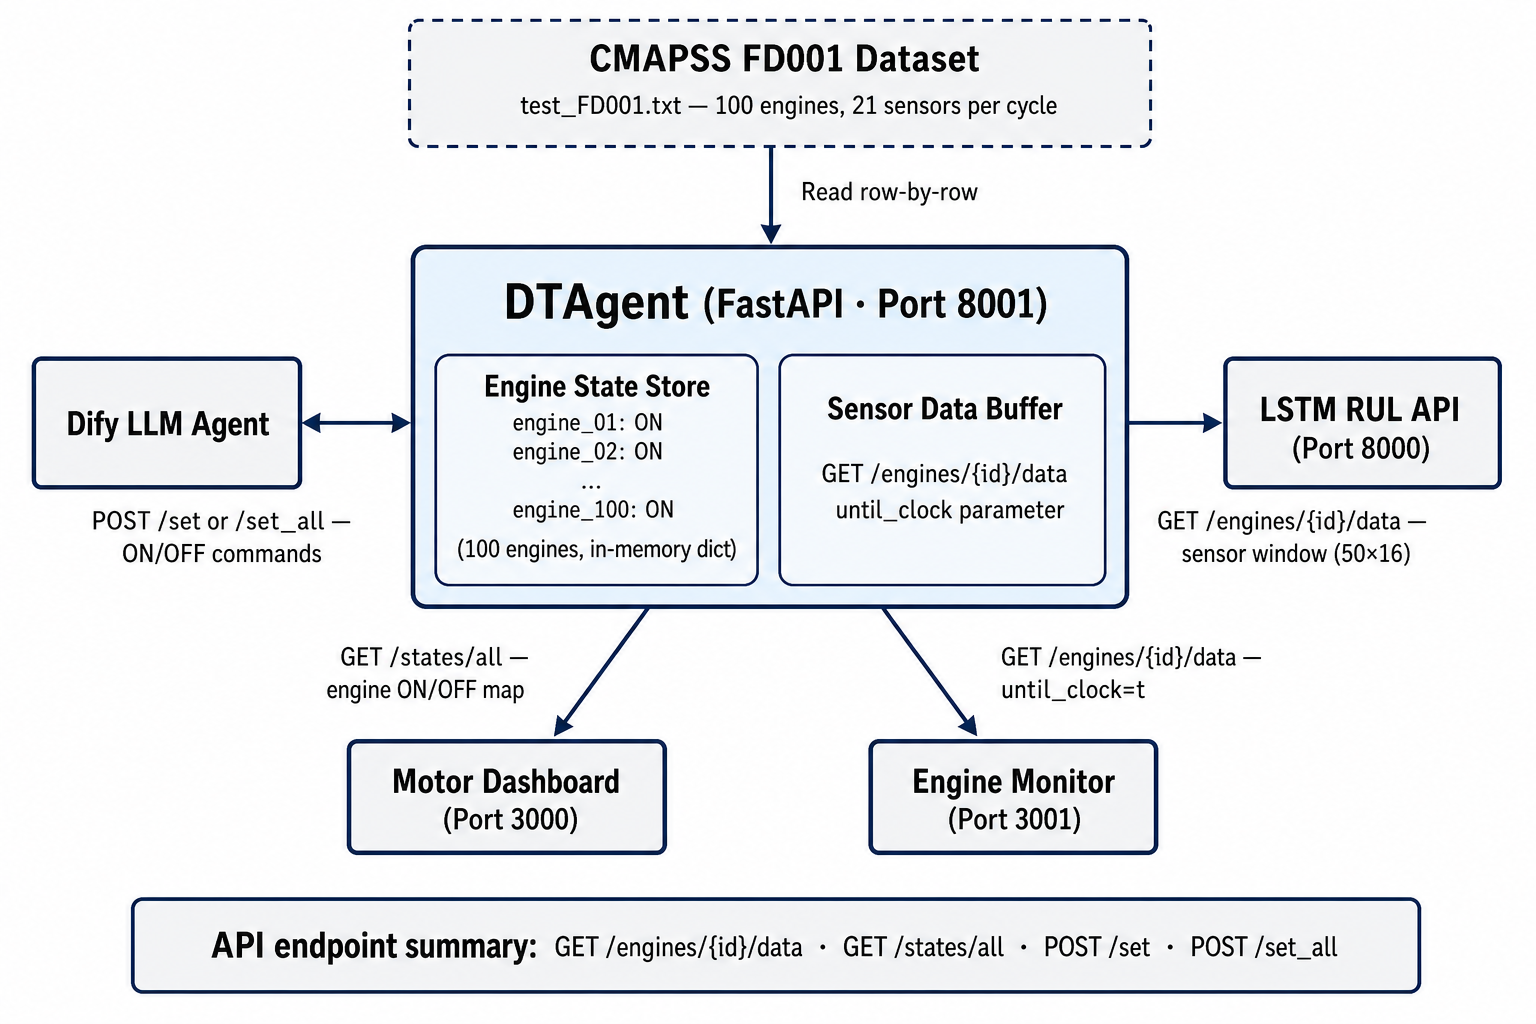
\includegraphics[width=0.92\textwidth]{images/agent_dtwin.png}
	\caption{نمای کلی ارتباطات بین عامل‌ها: دو هسته مرکزی (عامل دوقلو و عامل پیش‌بینی) داده را تأمین می‌کنند؛ سه واسط کاربری (عامل زبانی، عامل پایش، عامل \gls{Dashboard}) آن را مصرف می‌کنند \cite{marah2024madtwin}}
	\label{fig:impl-component}
\end{figure}

\subsection{سرویس‌ها و ماتریس یکپارچه‌سازی}

پنج سرویس سامانه با ترتیب مشخصی راه‌اندازی می‌شوند، زیرا وابستگی‌های راه‌اندازی وجود دارد: سرویس‌های هسته‌ای (عامل دوقلو و عامل پیش‌بینی) باید پیش از واسط‌های کاربری در دسترس باشند تا از خطای اتصال در لحظه راه‌اندازی جلوگیری شود. جدول \ref{tab:services-ports} ترتیب راه‌اندازی و پورت هر سرویس را نشان می‌دهد.

\begin{table}[ht]
	\centering
	\caption{مشخصات سرویس‌های سامانه و ترتیب راه‌اندازی}
	\label{tab:services-ports}
	\begin{tabular}{p{0.5cm}p{3.5cm}p{4cm}p{2.5cm}}
		\toprule
		\textbf{\#} & \textbf{نام سرویس} & \textbf{پوشه \lr{Compose}} & \textbf{پورت میزبان} \\
		\midrule
		۱ & عامل دوقلو (\lr{DTAgent}) & \lr{DTAgent/} & \lr{8001} \\
		۲ & عامل پیش‌بینی (\lr{lstm-rul-api}) & \lr{lstm-rul-api/} & \lr{8000} \\
		۳ & عامل زبانی (\lr{Dify}) & \lr{dify/docker/} & \lr{80/443} \\
		۴ & عامل \gls{Dashboard} (\lr{motor-dashboard}) & \lr{motor-dashboard/} & \lr{3000} \\
		۵ & عامل پایش (\lr{engine-monitor}) & \lr{engine-monitor/} & \lr{3001} \\
		\bottomrule
	\end{tabular}
\end{table}

همه سرویس‌ها از طریق \gls{Protocol} \lr{HTTP} با یکدیگر ارتباط برقرار می‌کنند. این انتخاب عمداً انجام شده: مرز بین سرویس‌ها با استفاده از \glspl{Protocol} \lr{REST} مشخص و مستند می‌شود و می‌توان هر سرویس را با پیاده‌سازی متفاوتی جایگزین کرد بدون اینکه سایر سرویس‌ها تحت تأثیر قرار گیرند. جدول \ref{tab:integration-matrix} ماتریس کامل این ارتباطات را نشان می‌دهد.

\begin{table}[ht]
	\centering
	\caption{ماتریس یکپارچه‌سازی بین سرویس‌ها}
	\label{tab:integration-matrix}
	\begin{tabular}{p{3.5cm}p{3.5cm}p{2cm}p{4.5cm}}
		\toprule
		\textbf{مبدأ} & \textbf{مقصد} & \textbf{قرارداد} & \textbf{پیکربندی} \\
		\midrule
		عامل زبانی & عامل پیش‌بینی & \lr{HTTP GET} & متغیر \lr{lstm\_host\_addr} \\
		\addlinespace
		عامل زبانی & عامل دوقلو & \lr{HTTP POST} & متغیر \lr{dt\_host\_addr} \\
		\addlinespace
		عامل پایش & عامل پیش‌بینی & \lr{HTTP GET} & \lr{REACT\_APP\_API\_BASE\_URL} \\
		\addlinespace
		عامل \gls{Dashboard} & عامل دوقلو & \lr{HTTP GET} & \lr{VITE\_API\_URL} \\
		\addlinespace
		\lr{docker-up.sh} & همه سرویس‌ها & \lr{Compose} & متغیر \lr{HOST\_IP} \\
		\bottomrule
	\end{tabular}
\end{table}

نکته قابل توجه در این ماتریس آن است که عامل زبانی تنها عاملی است که هم دسترسی خواندنی (از عامل پیش‌بینی) و هم دسترسی نوشتنی (به عامل دوقلو) دارد؛ این امر، عامل زبانی را به تنها حلقه تصمیم‌گیری در سامانه تبدیل می‌کند.


% -----------------------------------------------------------------------
\section{روش استقرار}\label{sec:deployment}

استقرار سامانه از طریق \gls{Script} \lr{docker-up.sh} انجام می‌شود که پنج فایل \lr{Docker Compose} را به‌ترتیب راه‌اندازی می‌کند. این رویکرد به جای یک فایل \lr{Compose} یکپارچه، انعطاف بیشتری در مدیریت چرخه حیات هر سرویس فراهم می‌کند: می‌توان تنها یک سرویس را راه‌اندازی مجدد کرد بدون اینکه کل سامانه قطع شود.

متغیر محیطی \lr{HOST\_IP} نقش کلیدی دارد. برخلاف \lr{localhost} که تنها در شبکه داخلی \lr{Docker} معنا دارد، \lr{HOST\_IP} آدرس آی‌پی قابل‌دسترس از شبکه محلی میزبان است. این آدرس هم در مرورگر \glspl{Client} (برای دسترسی به رابط‌های کاربری) و هم در گره‌های \lr{HTTP} عامل زبانی (که درون \gls{Container} \lr{Dify} اجرا می‌شوند) باید قابل‌رسیدن باشد. مقداردهی نادرست این متغیر رایج‌ترین مشکل در استقرار اولیه سامانه است.

از منظر زیرساخت، سامانه آزمایشگاهی نیازمند سامانه عامل لینوکس با \lr{Docker Engine}، یک آدرس آی‌پی ثابت در شبکه و \lr{RAM} کافی برای بارگذاری مدل \lr{TensorFlow} در حافظه است. آموزش مدل \gls{LSTM} که منبع‌بری‌ترین بخش است، جداگانه روی \lr{GPU} از طریق \lr{Google Colab} انجام شده و وزن‌های آموزش‌دیده به‌صورت فایل در سرویس پیش‌بینی استقرار می‌یابند؛ بنابراین استقرار اجرایی نیازی به \lr{GPU} ندارد.


% -----------------------------------------------------------------------
\section{عامل دوقلوی دیجیتال}\label{sec:impl-dtwin}

\subsection{نقش در معماری}

عامل دوقلوی دیجیتال از نظر معماری منحصربه‌فرد است: برخلاف چهار عامل دیگر که هر کدام یک لایه را می‌پوشانند، این سرویس همزمان دو لایه از معماری پنج‌لایه را تحقق می‌بخشد. از یک سو، به‌عنوان \gls{DataCollectionLayer} عمل می‌کند و داده خام حسگری را از فایل \gls{CMAPSS} به سایر سرویس‌ها ارائه می‌دهد؛ از سوی دیگر، به‌عنوان \gls{DigitalTwinAgentsLayer} وضعیت کنترلی \lr{ON/OFF} هر موتور را در حافظه نگه‌داری می‌کند. این دوگانگی در پیاده‌سازی‌های آزمایشگاهی امری طبیعی است و در نگاشت لایه‌های فصل سوم (جدول \ref{tab:layer-mapping}) صریحاً توضیح داده شده است.

مدل وضعیت موتور ساده اما مؤثر است. هر موتور با شناسه صحیح $k \in \{1, \ldots, N\}$ دارای یک حالت گسسته است:
\[
s_k \in \{\mathrm{ON},\,\mathrm{OFF}\}, \qquad k = 1, \ldots, 100
\]
در راه‌اندازی، همه موتورهای موجود در فایل آزمون \gls{CMAPSS} به حالت \lr{ON} مقداردهی می‌شوند؛ این فرض با سناریوی واقعی‌گرایانه‌تری هم‌خوان است که در آن همه موتورها تا قبل از دریافت فرمان صریح فعال فرض می‌شوند. تغییر حالت می‌تواند انتخابی (برای مجموعه $\mathcal{K}$ از شناسه‌ها) یا سراسری (برای همه موتورها) باشد.

\subsection{معماری سرویس}

همان‌طور که در شکل \ref{fig:impl-dtwin-arch} مشاهده می‌شود، سرویس از سه بخش اصلی تشکیل شده است. بخش اول پایگاه داده درون‌فرآیندی وضعیت موتورها است که به‌صورت یک \gls{Dict} ساده \lr{Python} (\lr{Dict[int, str]}) پیاده‌سازی شده. بخش دوم \gls{Cache} داده حسگری است که داده‌های خوانده‌شده از فایل \gls{CMAPSS} را در حافظه نگه می‌دارد تا از خواندن مکرر دیسک در هر درخواست جلوگیری شود. بخش سوم رابط \lr{REST API} است که هر دو جریان داده‌ای (حسگری خواندنی) و کنترلی (وضعیت نوشتنی) را از طریق نقاط پایانی تعریف‌شده در معرض سایر سرویس‌ها قرار می‌دهد.

\begin{figure}[H]
	\centering
	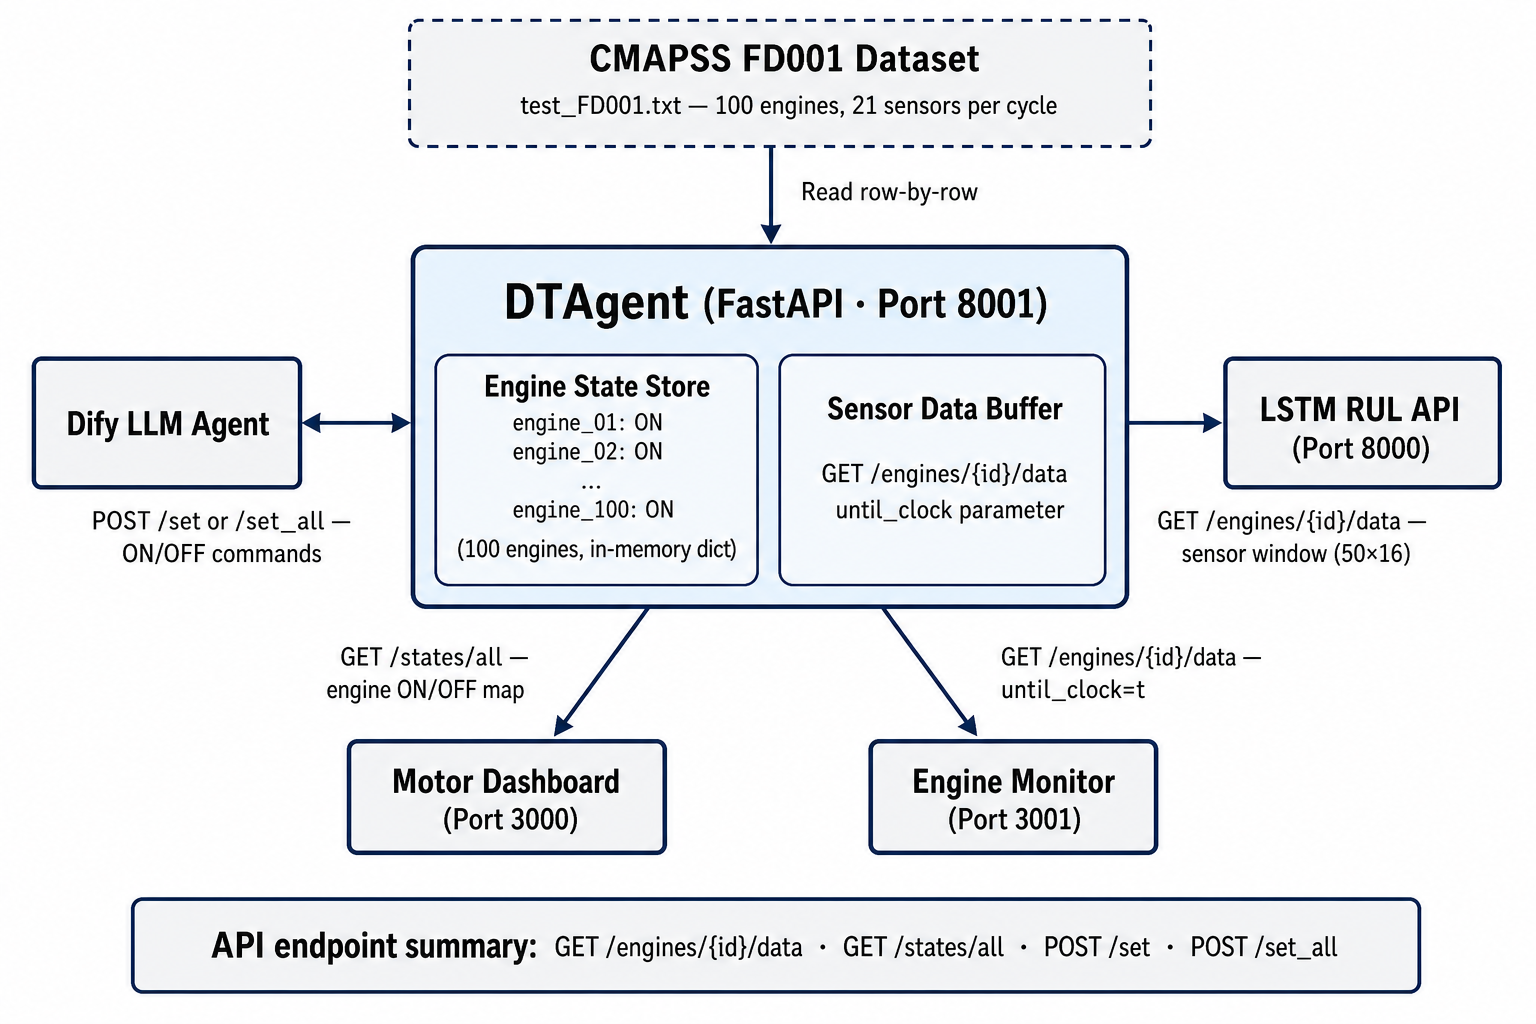
\includegraphics[width=0.90\textwidth]{images/agent_dtwin.png}
	\caption{معماری پیاده‌سازی عامل دوقلوی دیجیتال: داده خام \gls{CMAPSS} از طریق \lr{API} با پارامتر \lr{until\_clock} در اختیار عامل‌های مصرف‌کننده قرار می‌گیرد؛ فرمان‌های \lr{ON/OFF} از عامل زبانی دریافت می‌شوند؛ وضعیت ناوگان به عامل \gls{Dashboard} ارائه می‌شود \cite{marah2024madtwin}}
	\label{fig:impl-dtwin-arch}
\end{figure}

سرویس از معماری لایه‌ای \lr{FastAPI} با جداسازی مسئولیت‌ها پیروی می‌کند:
\begin{latin}
\begin{verbatim}
DTAgent/
├── app/
│   ├── main.py                 # CORS, startup, root endpoint
│   ├── api/routes_engine.py    # all /engines endpoints
│   ├── services/engine_service.py
│   ├── models/engine_state.py  # engine_states: Dict[int, str]
│   └── core/config.py          # TEST_DATA_PATH
├── Dockerfile                  # EXPOSE 8001
└── docker-compose.yaml
\end{verbatim}
\end{latin}

این ساختار لایه‌بندی شده اطمینان می‌دهد که منطق سرویس از تعریف مسیرها جدا است و آزمون‌پذیری سرویس افزایش می‌یابد.

\subsection{رابط برنامه‌نویسی}

رابط برنامه‌نویسی این سرویس پنج نقطه پایانی دارد که دو گروه عملکردی متمایز را پوشش می‌دهند. گروه اول نقاط پایانی خواندنی‌اند که داده حسگری یا وضعیت ناوگان را برمی‌گردانند. گروه دوم نقاط پایانی نوشتنی‌اند که وضعیت \lr{ON/OFF} را تغییر می‌دهند و تنها عامل زبانی مجاز به فراخوانی آن‌هاست. جدول \ref{tab:dtwin-api} این نقاط پایانی را به تفکیک نشان می‌دهد.

\begin{table}[ht]
	\centering
	\caption{نقاط پایانی رابط برنامه‌نویسی عامل دوقلوی دیجیتال}
	\label{tab:dtwin-api}
	\begin{tabular}{p{1.2cm}p{5cm}p{3cm}p{3.5cm}}
		\toprule
		\textbf{متد} & \textbf{مسیر} & \textbf{ورودی} & \textbf{خروجی} \\
		\midrule
		\lr{GET} & \lr{/engines/\{engine\_number\}} & \lr{until\_clock?: int} & \lr{records:[...]} حسگری \\
		\addlinespace
		\lr{GET} & \lr{/engines/states/all} & --- & فهرست \lr{\{engine\_number, state\}} \\
		\addlinespace
		\lr{POST} & \lr{/engines/states/set?state=ON|OFF} & بدنه: \lr{[1,3,5]} & \lr{updated\_states} \\
		\addlinespace
		\lr{POST} & \lr{/engines/states/set\_all?state=ON|OFF} & پارامتر کوئری & همه وضعیت‌ها \\
		\addlinespace
		\lr{GET} & \lr{/} & --- & پیام سلامت \\
		\bottomrule
	\end{tabular}
\end{table}

پارامتر \lr{until\_clock} در نقطه پایانی \lr{GET /engines/\{id\}} از نظر طراحی مهم‌ترین بخش رابط برنامه‌نویسی این سرویس است. این پارامتر به عامل پایش اجازه می‌دهد داده تنها تا لحظه شبیه‌سازی‌شده $t$ را درخواست کند؛ بدین ترتیب ماهیت زمان‌مند داده سری زمانی در محیط آزمایشگاهی بدون نیاز به \lr{streaming} واقعی شبیه‌سازی می‌شود. کد مقداردهی اولیه سرویس در لحظه راه‌اندازی به شرح زیر است:

\begin{latin}
\begin{verbatim}
@app.on_event("startup")
async def startup_event():
    initialize_engine_states()

def initialize_engine_states():
    df = get_data()
    unique_engines = df['unit_number'].unique()
    for eid in unique_engines:
        engine_states[int(eid)] = "ON"
\end{verbatim}
\end{latin}

این رویکرد تضمین می‌کند که حافظه وضعیت در لحظه راه‌اندازی \gls{Container} ساخته می‌شود و پاسخ به اولین درخواست بدون تأخیر مقداردهی امکان‌پذیر است.

\subsection{یکپارچه‌سازی و محدودیت‌های طراحی}

سه سرویس این \lr{API} را مصرف می‌کنند، هر کدام با الگوی متفاوتی: عامل \gls{Dashboard} وضعیت ناوگان را با نظرسنجی دوره‌ای می‌خواند، عامل زبانی پس از شناسایی موتورهای در خطر فرمان \lr{OFF} صادر می‌کند و عامل پایش داده حسگری تا افق زمانی مشخص را درخواست می‌کند. این تنوع در الگوهای مصرف یکی از شواهد اصلی است که نشان می‌دهد یک \lr{API} طراحی‌شده به‌درستی چگونه می‌تواند نیازهای متفاوت عامل‌های مختلف را پاسخ دهد.

محدودیت اصلی این سرویس عدم پایداری وضعیت است: چون وضعیت \lr{ON/OFF} موتورها درون حافظه فرآیند نگه‌داری می‌شود، راه‌اندازی مجدد \gls{Container} همه وضعیت‌ها را به \lr{ON} بازمی‌گرداند. در بستر آزمایشگاهی این رفتار قابل قبول بلکه مطلوب است، چون \glspl{Demo} می‌توانند از حالت اولیه شناخته‌شده شروع کنند. اما برای استقرار صنعتی واقعی، این وضعیت باید در یک پایگاه داده پایدار مانند \lr{Redis} ذخیره شود.


% -----------------------------------------------------------------------
\section{عامل پیش‌بینی عمر مفید باقیمانده}\label{sec:impl-lstm}

\subsection{آموزش مدل}

آموزش مدل با استفاده از دفترچه \lr{main\_lstm\_1\_v3\_loss\_function\_changed.ipynb} روی داده \gls{CMAPSS}-\lr{FD001} انجام شده است. پیش از آموزش، داده خام باید آماده‌سازی شود تا ویژگی‌های بی‌اطلاع یا تکراری حذف و دنباله‌های زمانی مناسب ساخته شوند.

مرحله اول آماده‌سازی، حذف ستون‌های فاقد اطلاعات است. هفت ستون \lr{TRA}، \lr{T2}، \lr{P2}، \lr{epr}، \lr{farB}، \lr{Nf\_dmd} و \lr{PCNfR\_dmd} در تمام نمونه‌های آموزشی مقدار ثابت دارند و هیچ اطلاعاتی برای مدل فراهم نمی‌کنند؛ حذف این ستون‌ها ابعاد ورودی را کاهش می‌دهد بدون اینکه اطلاعاتی از دست برود. در مرحله بعد، ستون‌های \lr{setting\_1}، \lr{setting\_2}، \lr{P15} و \lr{NRc} بر اساس تحلیل همبستگی حذف می‌شوند؛ این ستون‌ها یا همبستگی پایینی با خروجی \gls{RUL} دارند یا با سایر ویژگی‌های باقی‌مانده به‌حدی همبسته‌اند که اطلاعات جدیدی اضافه نمی‌کنند. شکل \ref{fig:correlation-heatmap} ماتریس هم‌بستگی را نشان می‌دهد که این تصمیم‌های انتخاب ویژگی را مستند می‌کند.

\begin{figure}[H]
	\centering
	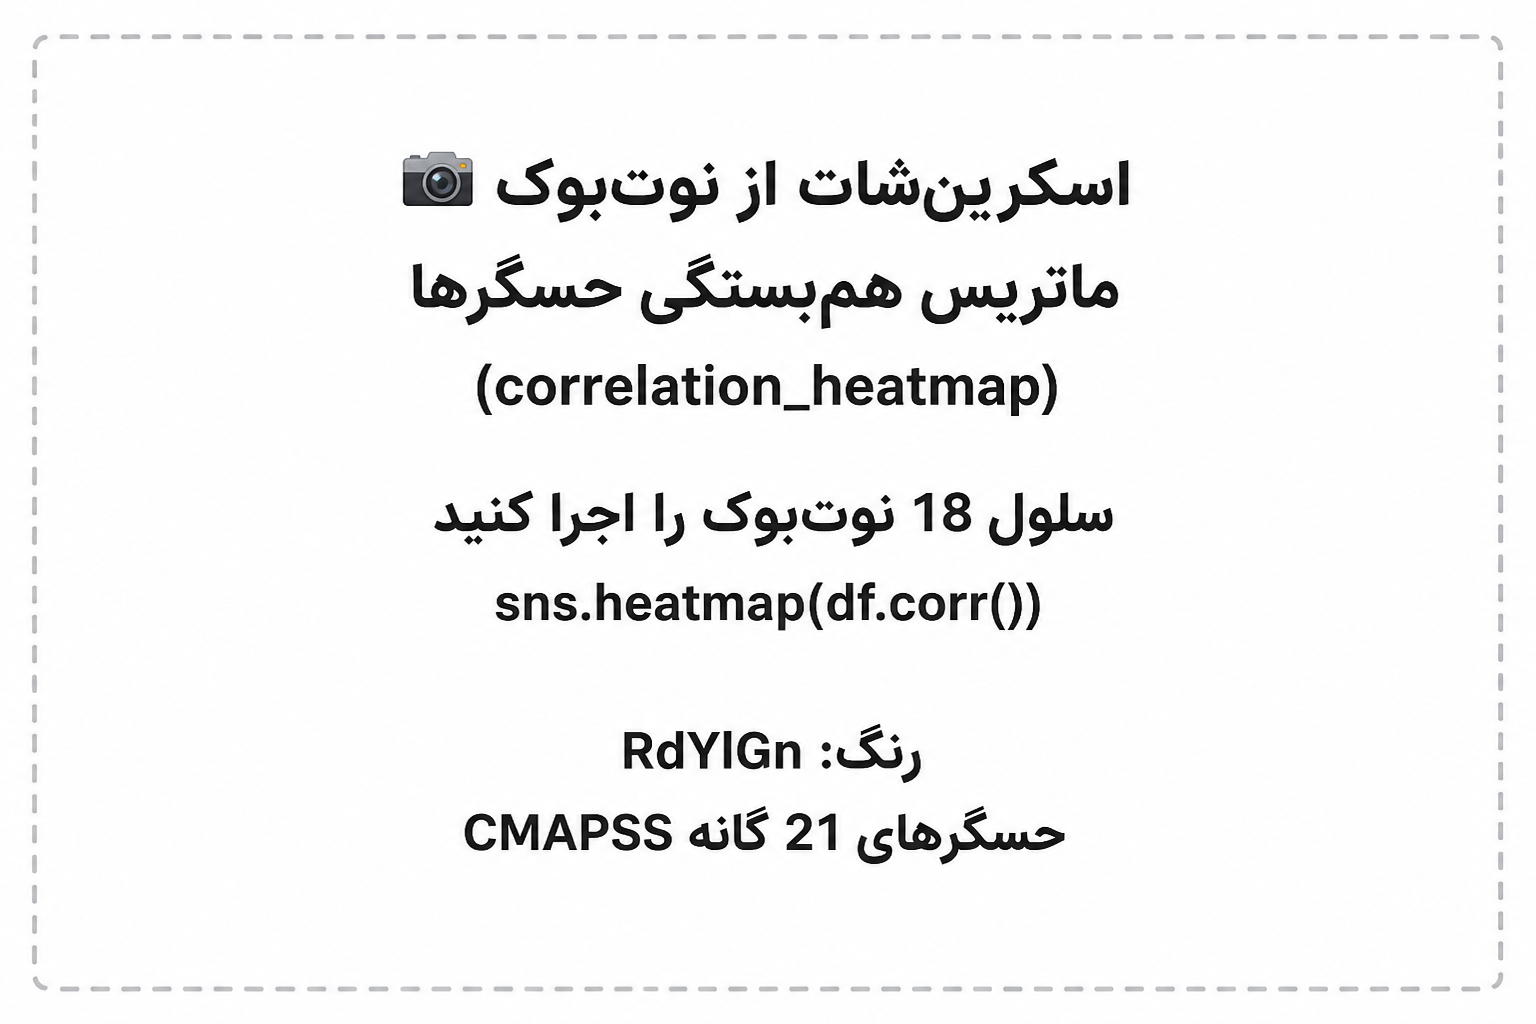
\includegraphics[width=0.85\textwidth]{images/correlation_heatmap.png}
	\caption{ماتریس هم‌بستگی حسگرهای \gls{CMAPSS} روی داده \lr{FD001}: مقادیر قرمز تیره نشان‌دهنده همبستگی بالا و کاندیدهای حذف هستند؛ این تحلیل مبنای کاهش ۲۱ حسگر اولیه به ۱۳ حسگر منتخب است [اسکرین‌شات از نوت‌بوک، سلول ۱۸]}
	\label{fig:correlation-heatmap}
\end{figure}

پس از انتخاب ویژگی، برچسب‌گذاری \gls{RUL} انجام می‌شود. برای داده آموزش، \gls{RUL} به‌صورت \(y^{(i)}(t) = t^{(i)}_\mathrm{end} - t\) محاسبه می‌شود؛ توجه می‌شود که برخلاف برخی پژوهش‌ها، سقف‌گذاری (piecewise clipping) اعمال نشده است. این انتخاب با \gls{PinballLoss} هم‌راستاست: سقف‌گذاری مصنوعی ممکن است نگاشت پیچیده‌تری از ویژگی به \gls{RUL} ایجاد کند. سپس هنجارسازی \lr{Min-Max} روی حسگرها اعمال می‌شود، با این محدودیت مهم که پارامترهای هنجارسازی منحصراً از داده آموزش استخراج می‌شوند و روی داده آزمون نیز اعمال می‌گردند تا از نشت اطلاعات (data leakage) جلوگیری شود. در گام پایانی، ویژگی \lr{cycle\_norm} --- شماره چرخه هنجارشده به بازه $[0,1]$ --- به‌عنوان یک ویژگی زمانی مستقل اضافه می‌شود. این ویژگی به مدل کمک می‌کند موقعیت نسبی موتور در چرخه عمرش را درک کند، نه تنها وضعیت لحظه‌ای حسگرها را.

ساخت پنجره‌های لغزنده آخرین گام آماده‌سازی است. برای هر موتور، توالی‌هایی به طول $w=50$ گام زمانی ساخته می‌شود؛ موتورهایی که تعداد چرخه کمتری از ۵۰ دارند با صفرگذاری (zero-padding) در ابتدای توالی تکمیل می‌شوند تا شکل ورودی یکنواخت باشد. ویژگی‌های توالی نهایی ۱۶ ستون دارند:

\begin{latin}
\begin{verbatim}
unit_number, time_in_cycles, T24, T30, T50, P30, Nf, Nc,
Ps30, phi, NRf, BPR, htBleed, W31, W32, cycle_norm
\end{verbatim}
\end{latin}

از این ۱۶ ویژگی، \lr{unit\_number} و \lr{time\_in\_cycles} بدون هنجارسازی وارد می‌شوند؛ ۱۳ حسگر منتخب با \lr{Min-Max} هنجار می‌شوند؛ و \lr{cycle\_norm} پیشاپیش در بازه $[0,1]$ است.

معماری شبکه عصبی در جدول \ref{tab:lstm-arch} نشان داده شده است. شبکه از دو لایه \gls{LSTM} تشکیل شده که هر دو با \lr{return\_sequences=True} تمام دنباله را به لایه بعدی می‌دهند. این تنظیم برای لایه توجه ضروری است که باید به هر گام زمانی دسترسی داشته باشد تا وزن‌های $\alpha_t$ را محاسبه کند. لایه‌های \lr{Dropout} با نرخ ۰٫۲ بین هر جفت لایه \gls{LSTM} و توجه قرار گرفته‌اند تا \lr{overfitting} را کنترل کنند. مجموع ۷۷٬۱۵۱ پارامتر قابل آموزش نشان می‌دهد که مدل به‌اندازه کافی ظرفیت دارد بدون اینکه بیش از حد پیچیده باشد.

\begin{table}[ht]
	\centering
	\caption{معماری شبکه عصبی عامل پیش‌بینی (نسخه \lr{V3})}
	\label{tab:lstm-arch}
	\begin{tabular}{p{3.5cm}p{5cm}p{5cm}}
		\toprule
		\textbf{لایه} & \textbf{مشخصات} & \textbf{توضیح} \\
		\midrule
		\lr{Input} & شکل $50 \times 16$ & ۵۰ گام زمانی، ۱۶ ویژگی \\
		\lr{LSTM-1} & ۱۰۰ واحد، \lr{return\_sequences=True} & دنباله کامل خروجی می‌دهد \\
		\lr{Dropout-1} & نرخ ۰٫۲ & منظم‌کننده \\
		\lr{LSTM-2} & ۵۰ واحد، \lr{return\_sequences=True} & دنباله کامل خروجی می‌دهد \\
		\lr{Dropout-2} & نرخ ۰٫۲ & منظم‌کننده \\
		\gls{AttentionLayer} & وزن‌های زمانی $\alpha_t$ & بردار زمینه $\mathbf{c} = \sum_t \alpha_t h_t$ \\
		\lr{Dense} & ۱ واحد، فعال‌سازی خطی & خروجی اسکالر \gls{RUL} \\
		\addlinespace
		\multicolumn{2}{l}{\textbf{تعداد کل پارامترها:}} & $77{,}151$ \\
		\bottomrule
	\end{tabular}
\end{table}

انتخاب \glspl{Hyperparameter} در جدول \ref{tab:lstm-hyperparams} آمده است. بهینه‌ساز \lr{RMSprop} برای داده‌های سری زمانی توصیه‌شده است و در مقایسه با \lr{Adam} در برخی آزمایش‌ها پایداری بهتری نشان می‌دهد. اندازه دسته ۲۰۰ نسبت به اندازه مجموعه داده آموزشی (۲۰٬۶۳۱ نمونه) معقول است و نسبت اعتبارسنجی ۵\% به مجموعه اعتبارسنجی ۱٬۰۳۲ نمونه‌ای می‌دهد که برای پایش \lr{overfitting} کافی است.

\begin{table}[ht]
	\centering
	\caption{\glspl{Hyperparameter} آموزش مدل \lr{LSTM} (نسخه \lr{V3})}
	\label{tab:lstm-hyperparams}
	\begin{tabular}{p{5cm}p{8.5cm}}
		\toprule
		\textbf{پارامتر} & \textbf{مقدار} \\
		\midrule
		بهینه‌ساز & \lr{RMSprop} (نرخ یادگیری پیش‌فرض ≈$0.001$) \\
		اندازه دسته & ۲۰۰ \\
		تعداد دوره آموزش & ۶۰ \\
		نسبت اعتبارسنجی & ۰٫۰۵ \\
		تابع زیان & \lr{PinballLoss} ($\tau = 0.125$) \\
		معیارهای پایش & \lr{MAE}، $R^2$ سفارشی \\
		\bottomrule
	\end{tabular}
\end{table}

تابع زیان \gls{PinballLoss} با $\tau = 0.125$ --- که در فصل سوم در رابطه \eqref{eq:pinball-loss} تعریف شد --- نوآوری اصلی آموزش این مدل است. با این انتخاب، ضریب جریمه بیش‌برآورد ($\hat{y} > y$) برابر $0.875$ و ضریب جریمه کم‌برآورد ($\hat{y} < y$) تنها $0.125$ است؛ یعنی مدل در شرایط عدم‌قطعیت قوی‌ترین محرک را برای کم برآورد کردن \gls{RUL} دارد. نتیجه عملی این طراحی در فصل پنجم بررسی می‌شود.

شکل \ref{fig:train-curves} منحنی‌های آموزش مدل \lr{V3} را در ۶۰ دوره نشان می‌دهد. در نمودارهای \lr{Loss} و \lr{MAE}، هر دو منحنی آموزش و اعتبارسنجی روندی نزولی یکسان دارند و شکافی چشمگیر بین آن‌ها مشاهده نمی‌شود؛ این نشانه غیاب \lr{overfitting} و تعمیم‌پذیری مناسب مدل است.

\begin{figure}[H]
	\centering
	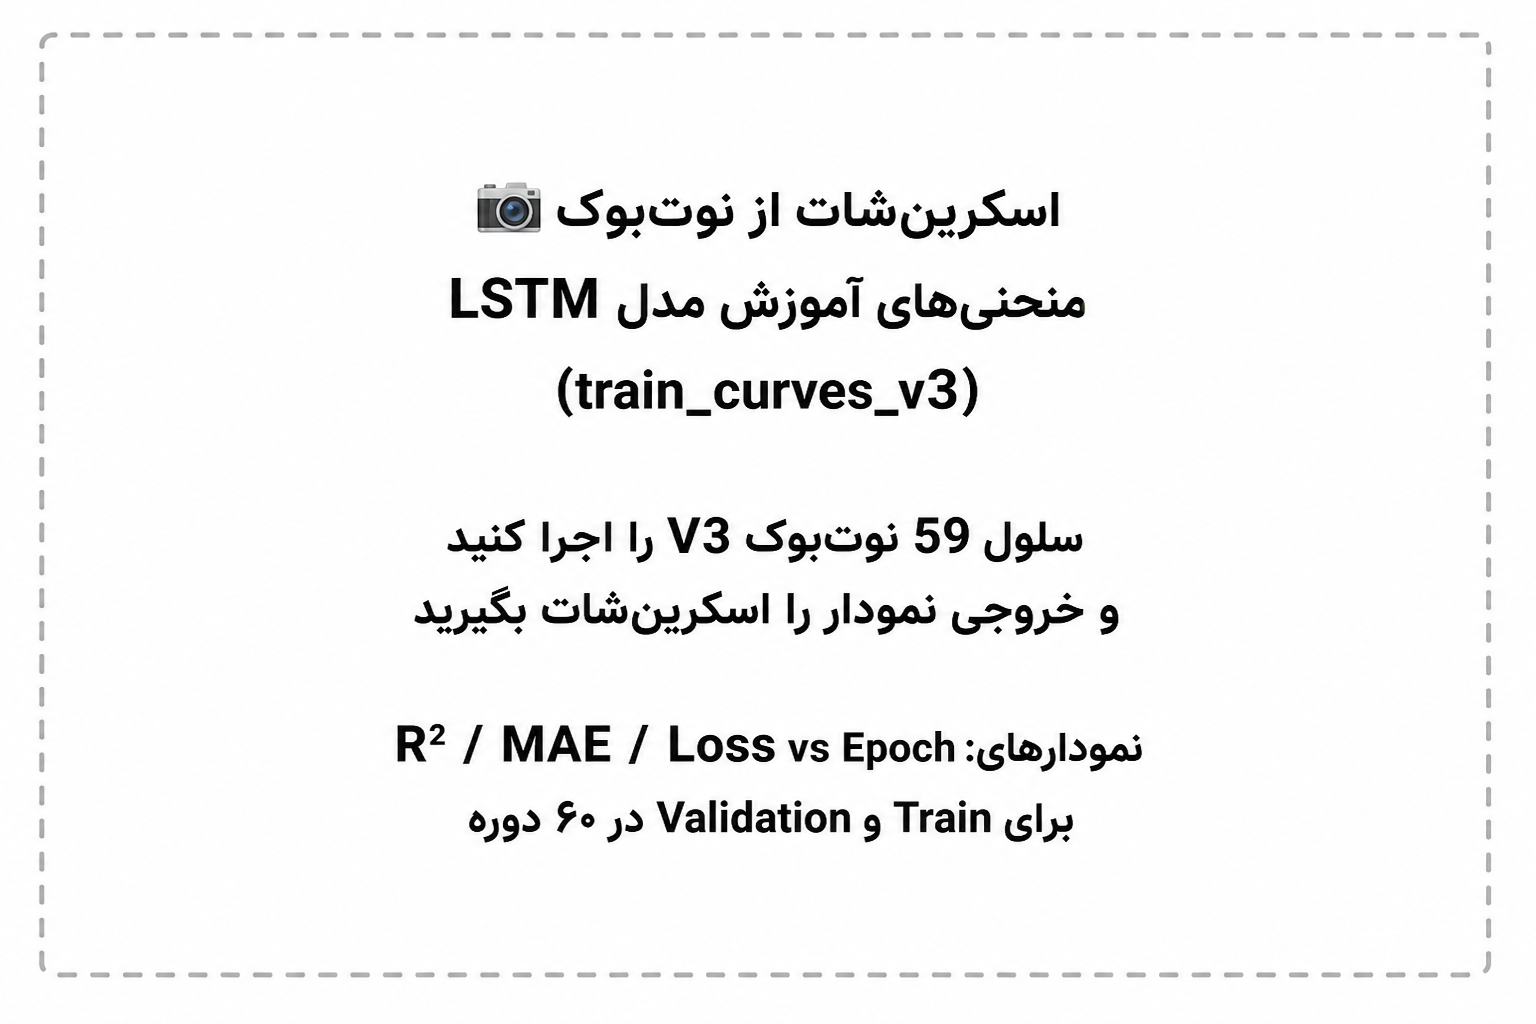
\includegraphics[width=0.90\textwidth]{images/train_curves_v3.png}
	\caption{منحنی‌های آموزش مدل \lr{V3}: همگرایی تدریجی \lr{Pinball Loss}، \lr{MAE} و $R^2$ برای مجموعه‌های آموزش و اعتبارسنجی در ۶۰ دوره؛ نبود شکاف میان دو منحنی نشانه تعمیم‌پذیری مناسب است [اسکرین‌شات از نوت‌بوک، سلول ۵۹]}
	\label{fig:train-curves}
\end{figure}

\subsection{سرویس پیش‌بینی}

مدل آموزش‌دیده پس از اتمام آموزش، به‌صورت یک سرویس \lr{REST API} مبتنی بر \lr{FastAPI} بسته‌بندی و مستقر می‌شود. شکل \ref{fig:impl-lstm-arch} مسیر داده درون این سرویس را نشان می‌دهد: ورودی یک تانسور توالی زمانی است و خروجی شامل دو قسمت است --- مقدار اسکالر \gls{RUL} و بردار اهمیت حسگرها که محصول جانبی \gls{AttentionLayer} است.

\begin{figure}[H]
	\centering
	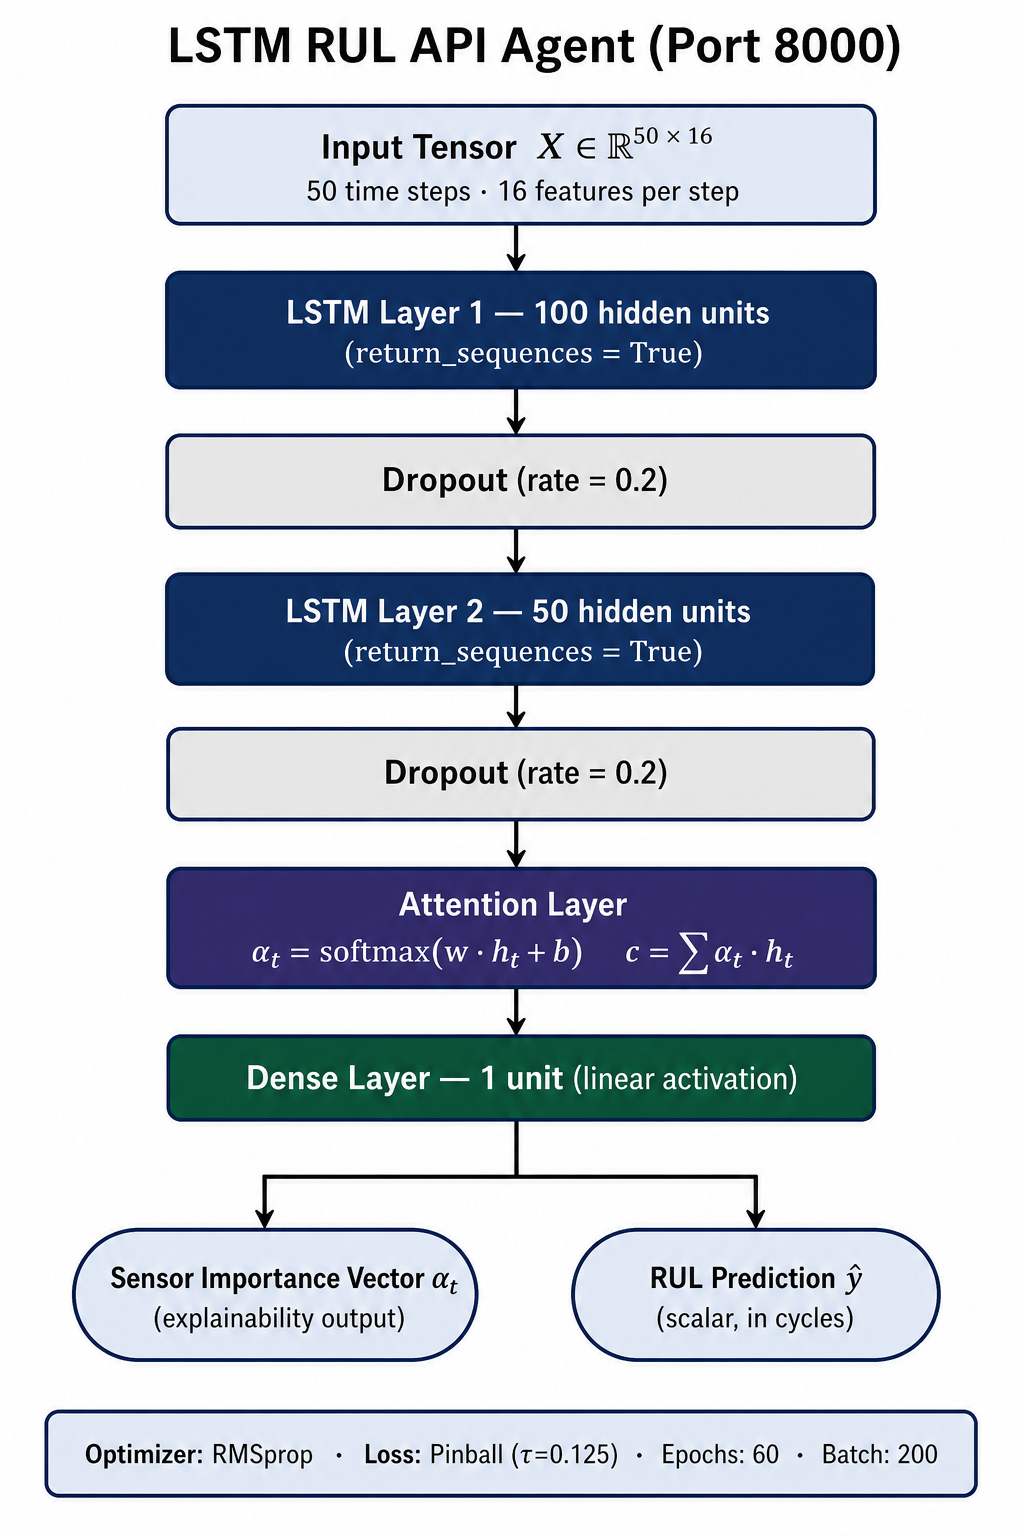
\includegraphics[width=0.60\textwidth]{images/agent_lstm_rul.png}
	\caption{معماری سرویس عامل پیش‌بینی: ورودی تانسور $(50\times16)$ از طریق لایه‌های \gls{LSTM} و توجه پردازش می‌شود و دو خروجی تولید می‌کند --- \gls{RUL} برای پایش و بردار اهمیت حسگرها برای توضیح‌پذیری}
	\label{fig:impl-lstm-arch}
\end{figure}

یکی از تصمیم‌های طراحی مهم بارگذاری مدل در لحظه راه‌اندازی سرویس است. این عملیات یک‌بار هنگام \lr{import} روتر انجام می‌شود تا تأخیر سرد (cold start) در اولین درخواست حذف شود. اگر بارگذاری با شکست مواجه شود، متغیر \lr{model} روی \lr{None} می‌ماند و همه نقاط پایانی پاسخ خطای نرم برمی‌گردانند بدون اینکه فرآیند \lr{crash} کند:

\begin{latin}
\begin{verbatim}
try:
    model, history, model_data = load_lstm_model(MODEL_BASE_PATH)
    lstm_test_df = model_data["lstm_test_df"]
    sequence_length = model_data["sequence_length"]
    sequence_cols = model_data["sequence_cols"]
except Exception as e:
    model = None   # endpoints return soft error
\end{verbatim}
\end{latin}

شیء \lr{AttentionLayer} و تابع \lr{r2\_keras} که هنگام آموزش تعریف شده‌اند به‌عنوان \lr{custom\_objects} به \lr{load\_model} پاس داده می‌شوند تا بارگذاری مدل سفارشی به‌درستی انجام شود. رابط برنامه‌نویسی این سرویس چهار نقطه پایانی دارد که در جدول \ref{tab:lstm-api} توضیح داده شده‌اند.

\begin{table}[ht]
	\centering
	\caption{نقاط پایانی رابط برنامه‌نویسی عامل پیش‌بینی}
	\label{tab:lstm-api}
	\begin{tabular}{p{1.2cm}p{6.5cm}p{5.5cm}}
		\toprule
		\textbf{متد} & \textbf{مسیر} & \textbf{توضیح} \\
		\midrule
		\lr{GET} & \lr{/api/health} & سلامت سرویس \\
		\addlinespace
		\lr{GET} & \lr{/api/predict/predict\_rul/\{engine\_number\}?k=5} & \gls{RUL} + \lr{top-k} حسگر مؤثر \\
		\addlinespace
		\lr{GET} & \lr{/api/predict/engines\_with\_low\_rul/?threshold=50\&until\_clock=} & فهرست موتورهای کم‌عمر با \gls{RUL} کمتر از آستانه \\
		\addlinespace
		\lr{POST} & \lr{/api/predict/predict\_new\_engine\_rul/} & پیش‌بینی روی توالی دلخواه \\
		\bottomrule
	\end{tabular}
\end{table}

نقطه پایانی \lr{predict\_rul} پرکاربردترین نقطه است که پس از دریافت شناسه موتور، توالی آماده‌شده را از فایل \gls{CMAPSS} می‌سازد، مدل را اجرا می‌کند و نتیجه را در قالب \lr{JSON} برمی‌گرداند. نمونه پاسخ زیر نشان می‌دهد که چگونه \gls{RUL} عددی در کنار بردار اهمیت حسگرها به‌صورت یکپارچه ارائه می‌شود:

\begin{latin}
\begin{verbatim}
{
  "engine_number": 10,
  "predicted_rul": 164.67,
  "sensor_impacts": [
    {"sensor": "T30",  "percent": 18.5},
    {"sensor": "Ps30", "percent": 12.1},
    {"sensor": "NRf",  "percent": 10.3}
  ]
}
\end{verbatim}
\end{latin}

\subsection{توضیح‌پذیری مبتنی بر توجه}

توضیح‌پذیری درون‌ذات یکی از مزایای معماری انتخاب‌شده است. برخلاف روش‌هایی مانند \lr{SHAP} که پس از آموزش و به‌صورت جداگانه اجرا می‌شوند، در این پیاده‌سازی اطلاعات توضیح‌پذیری مستقیماً از معماری شبکه استخراج می‌شوند. تابع \lr{get\_rul\_and\_attribution} خروجی میانی \gls{AttentionLayer} را می‌گیرد و وزن‌های زمانی $\alpha_t$ را به سهم هر حسگر تبدیل می‌کند. این تبدیل شامل \gls{Normalization} \lr{L1} روی بردار زمینه است؛ سپس شناسه‌های غیرحسی (\lr{unit\_number}، \lr{time\_in\_cycles}، \lr{cycle\_norm}) حذف می‌شوند و \lr{top-k} حسگر مؤثرترین به‌عنوان خروجی توضیح‌پذیری برای عامل زبانی ارسال می‌شود. این رویکرد تأخیر استنتاج را نسبت به \lr{SHAP} به میزان چشمگیری کاهش می‌دهد، چون محاسبه بردار اهمیت همراه با پیش‌بینی و در یک پاس رو به جلو انجام می‌شود.


% -----------------------------------------------------------------------
\section{عامل تعامل مدل زبانی}\label{sec:impl-llm}

\subsection{الگوی طراحی}

ادغام مدل‌های زبانی با سامانه‌های \glspl{Digital Twins} در ادبیات با دو رویکرد اصلی انجام می‌شود: حلقه \lr{ReAct} که \gls{LLM} به‌صورت پویا ابزار را انتخاب می‌کند، و \gls{Workflow} از پیش تعریف‌شده که \gls{LLM} درون یک گراف تصمیم ثابت قرار می‌گیرد. پژوهش حاضر رویکرد دوم را برگزیده است \cite{CHEN2025102982LLMDT,park2025interactive}. دلیل این انتخاب کنترل‌پذیری است: در یک سامانه صنعتی که با ایمنی موتور هوافضا سر و کار دارد، قابلیت پیش‌بینی رفتار \gls{LLM} اهمیت حیاتی دارد؛ کاربر باید بداند که «خاموش کردن موتورهای در خطر» همیشه دقیقاً همان توالی از اقدامات را اجرا می‌کند.

\begin{figure}[H]
	\centering
	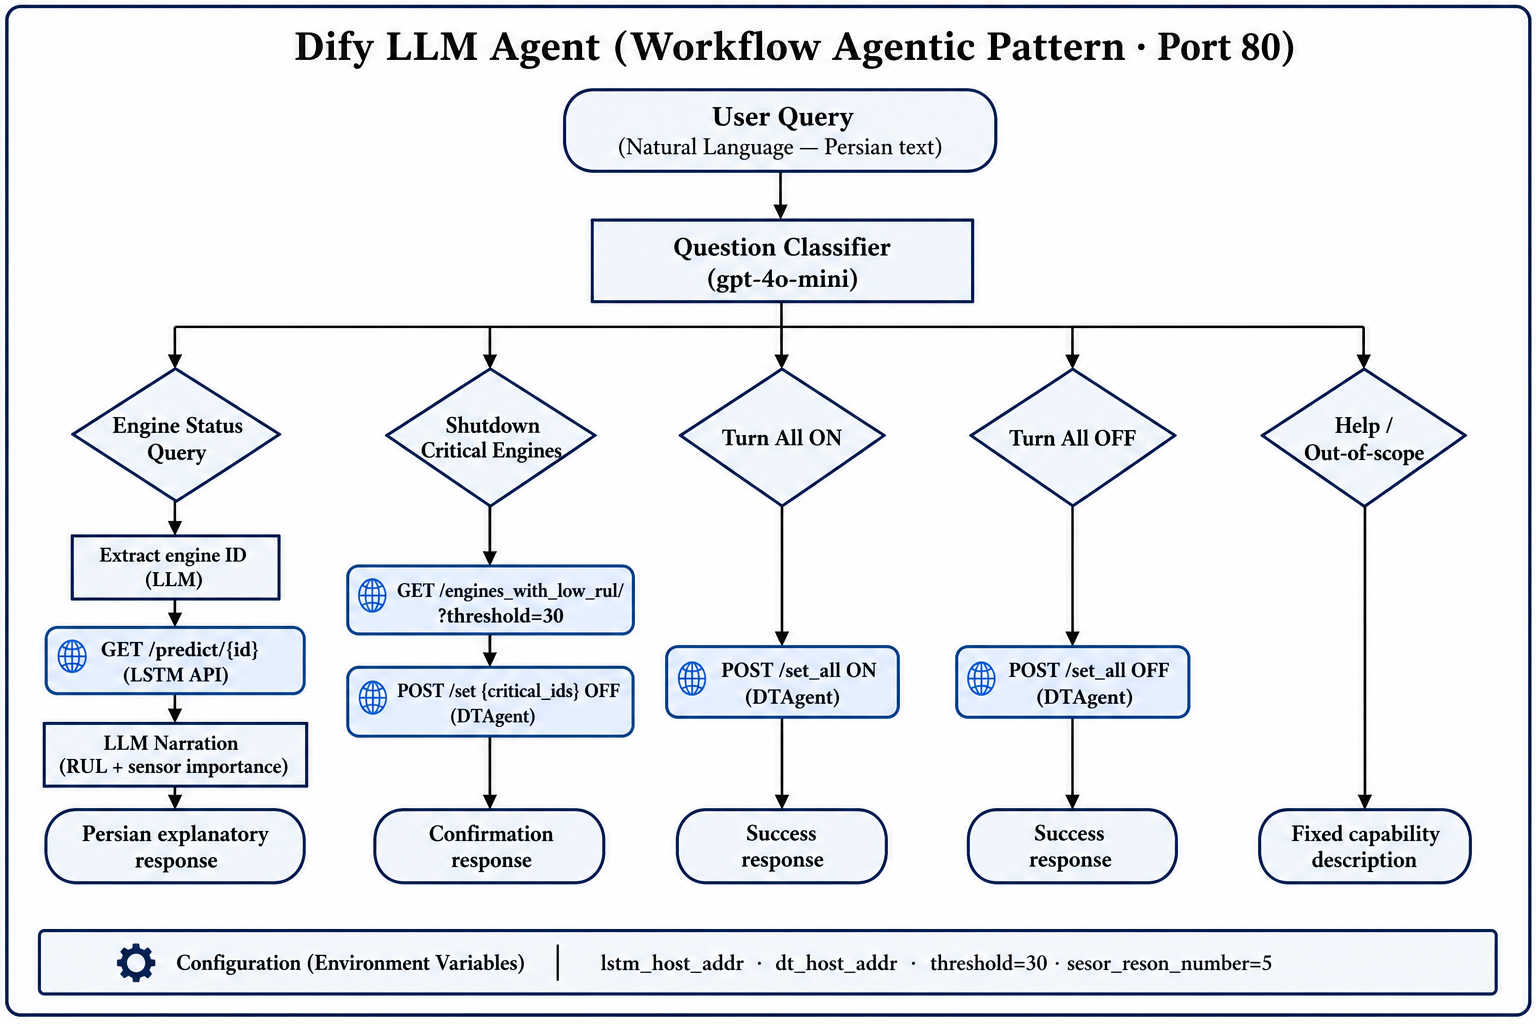
\includegraphics[width=0.90\textwidth]{images/agent_dify_llm.png}
	\caption{معماری سرویس عامل تعامل زبانی: طبقه‌بند نیت پنج شاخه قطعی دارد و در هر شاخه ترکیب مشخصی از گره‌های \lr{LLM} و \lr{HTTP} اجرا می‌شود؛ \gls{LLM} نقش طبقه‌بندی و روایت دارد نه تصمیم‌گیری مستقل \cite{CHEN2025102982LLMDT}}
	\label{fig:impl-llm-arch}
\end{figure}

\begin{figure}[H]
	\centering
	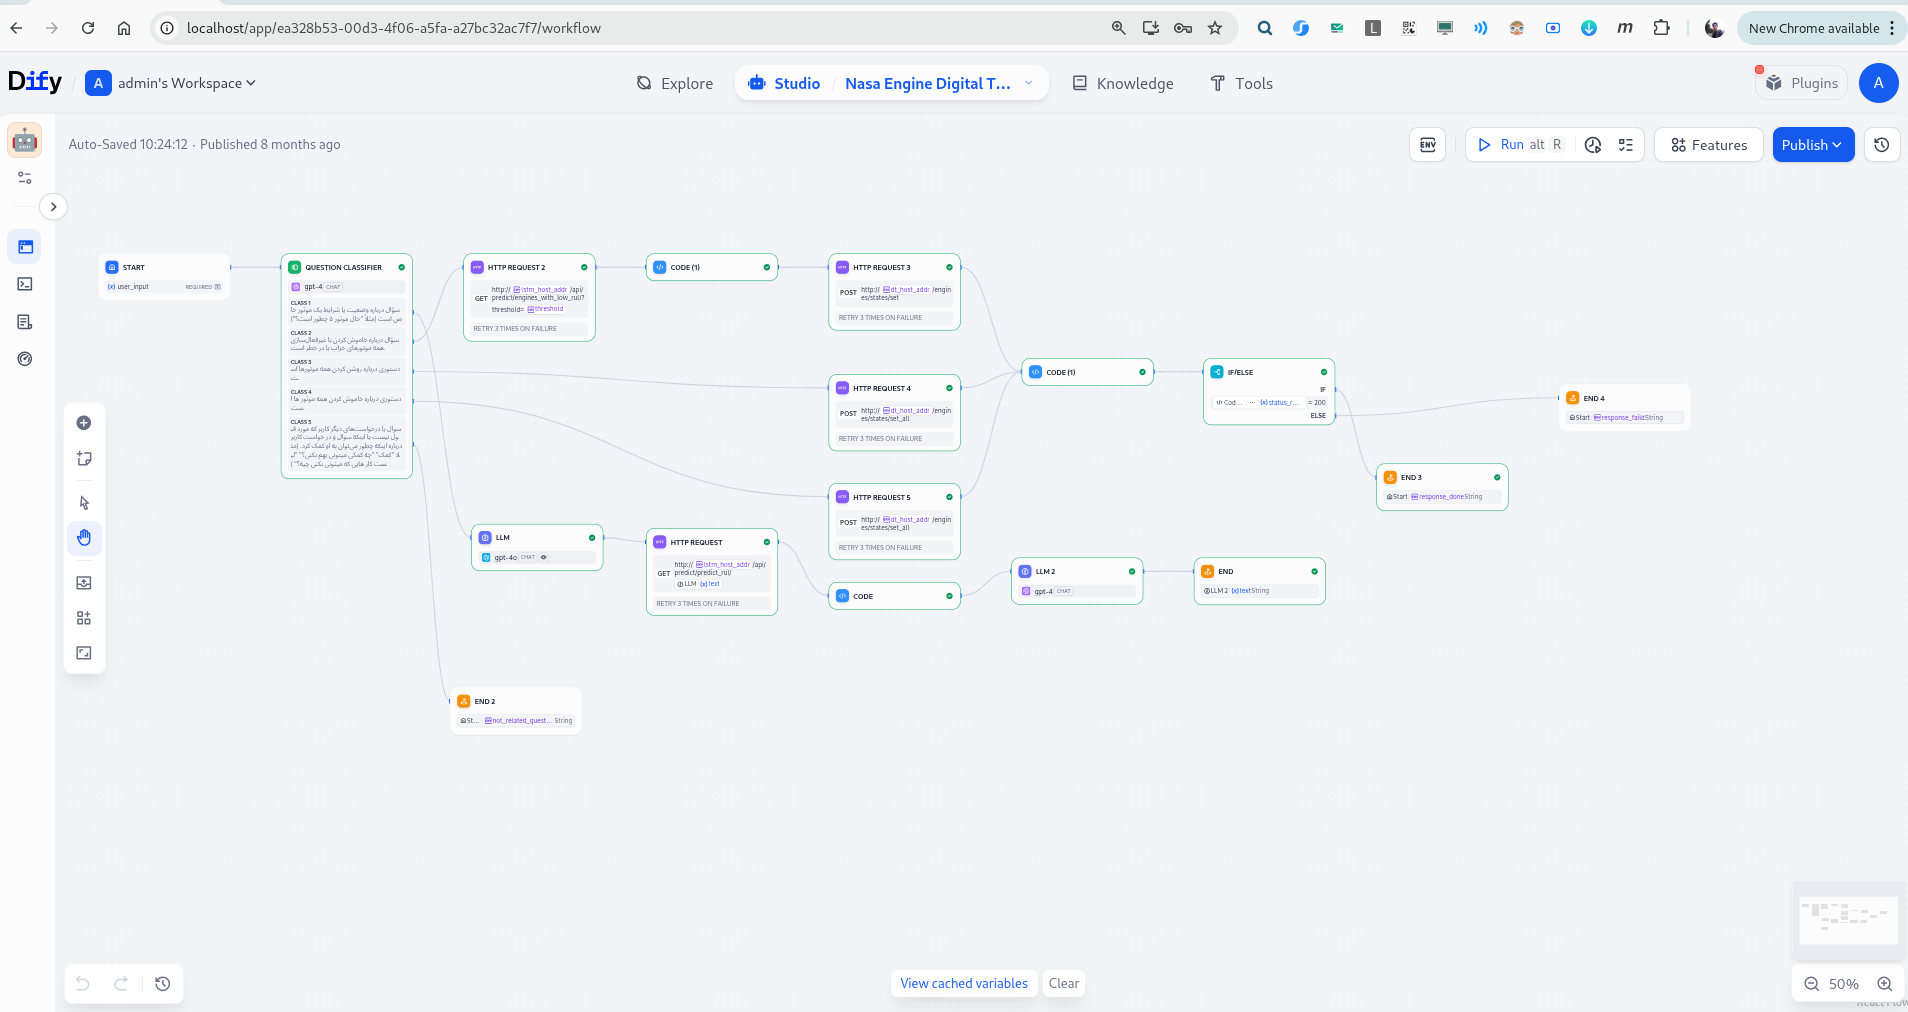
\includegraphics[width=0.92\textwidth]{images/dify_workflow_screenshot.png}
	\caption{گراف واقعی \gls{Workflow} عامل زبانی در \gls{Platform} \lr{Dify}: گره طبقه‌بند نیت در مرکز دیده می‌شود و پنج شاخه از آن منشعب می‌شوند؛ گره‌های \lr{HTTP} (آبی رنگ) ابزارهای فراخوانی سرویس‌های دیگر هستند}
	\label{fig:dify-workflow-screenshot}
\end{figure}

\subsection{فضای نیت و شاخه‌های تصمیم}

طراحی فضای نیت بر اساس تحلیل سناریوهای واقعی \glspl{Operator} ناوگان انجام شده است. یک \gls{Operator} معمولاً می‌خواهد یا وضعیت موتور خاصی را بداند، یا اقدامی روی ناوگان انجام دهد. این دو نوع تعامل پنج کلاس نیت ایجاد می‌کنند که در جدول \ref{tab:intent-space} با اقدام متناظر هر کلاس توضیح داده شده‌اند.

\begin{table}[ht]
	\centering
	\caption{فضای نیت عامل تعاملی و اقدام هر شاخه}
	\label{tab:intent-space}
	\begin{tabular}{p{0.6cm}p{3.5cm}p{4cm}p{5cm}}
		\toprule
		\textbf{\#} & \textbf{نیت} & \textbf{مثال ورودی} & \textbf{اقدام} \\
		\midrule
		۱ & وضعیت یک موتور & «موتور ۱ چه زمانی خراب می‌شود؟» & استخراج شناسه → \lr{GET predict\_rul/k} → روایت فارسی \\
		\addlinespace
		۲ & خاموش‌سازی موتورهای درخطر & «موتورهای در خطر را خاموش کن» & \lr{GET low\_rul} → \lr{POST set OFF} \\
		\addlinespace
		۳ & روشن کردن همه & «همه موتورها را روشن کن» & \lr{POST set\_all ON} \\
		\addlinespace
		۴ & خاموش کردن همه & «همه موتورها را خاموش کن» & \lr{POST set\_all OFF} \\
		\addlinespace
		۵ & راهنما / خارج از حوزه & «چه کمکی می‌توانی بکنی؟» & پاسخ ثابت معرفی قابلیت‌ها \\
		\bottomrule
	\end{tabular}
\end{table}

نکته قابل توجه آن است که کلاس‌های ۳ و ۴ (فرمان‌های سراسری) هیچ فراخوانی \gls{LLM} ندارند --- درخواست کاربر مستقیماً به یک فراخوان \lr{HTTP} به عامل دوقلو تبدیل می‌شود. این تمایز توضیح‌دهنده توزیع دوقله‌ای تأخیر پاسخ است که در فصل پنجم مشاهده می‌شود.

\subsection{گره‌های HTTP و متغیرهای محیطی}

هر شاخه تصمیم ترکیبی از گره‌های \lr{HTTP} دارد که به سرویس‌های زیرین متصل می‌شوند. جدول \ref{tab:http-nodes} پنج گره \lr{HTTP} تعریف‌شده در \gls{Workflow} را نشان می‌دهد. برنامه‌نویسی این گره‌ها در \gls{Platform} \lr{Dify} از طریق متغیرهای محیطی انجام می‌شود تا بدون نیاز به تغییر کد، آدرس سرویس‌ها یا آستانه‌های تصمیم قابل تنظیم باشند.

\begin{table}[ht]
	\centering
	\caption{گره‌های \lr{HTTP} \gls{Workflow} عامل زبانی}
	\label{tab:http-nodes}
	\begin{tabular}{p{1.5cm}p{6cm}p{6cm}}
		\toprule
		\textbf{متد} & \textbf{مسیر مفهومی} & \textbf{هدف} \\
		\midrule
		\lr{GET} & \lr{/api/predict/predict\_rul/\{id\}} & پیش‌بینی \gls{RUL} برای موتور مشخص \\
		\addlinespace
		\lr{GET} & \lr{/api/predict/engines\_with\_low\_rul/?threshold=} & فهرست موتورهای کم‌عمر \\
		\addlinespace
		\lr{POST} & \lr{/engines/states/set?state=OFF} + بدنه لیست & خاموش‌سازی انتخابی \\
		\addlinespace
		\lr{POST} & \lr{/engines/states/set\_all?state=ON} & روشن کردن سراسری \\
		\addlinespace
		\lr{POST} & \lr{/engines/states/set\_all?state=OFF} & خاموش کردن سراسری \\
		\bottomrule
	\end{tabular}
\end{table}

متغیرهای محیطی کلیدی که رفتار \gls{Workflow} را کنترل می‌کنند در جدول \ref{tab:env-vars} آمده‌اند. قابل توجه‌ترین متغیر \lr{threshold} است که آستانه تشخیص موتور «در خطر» را تعیین می‌کند. مقدار پیش‌فرض ۳۰ چرخه در عامل زبانی تعریف شده، در حالی که عامل پایش با آستانه پیش‌فرض ۵۰ کار می‌کند؛ این تفاوت در بخش محدودیت‌ها مورد بحث قرار می‌گیرد.

\begin{table}[ht]
	\centering
	\caption{متغیرهای محیطی کلیدی \gls{Workflow} عامل زبانی}
	\label{tab:env-vars}
	\begin{tabular}{p{4.5cm}p{3.5cm}p{5.5cm}}
		\toprule
		\textbf{متغیر} & \textbf{نمونه مقدار} & \textbf{نقش} \\
		\midrule
		\lr{lstm\_host\_addr} & \lr{10.226.63.45:8000} & آدرس عامل پیش‌بینی \\
		\lr{dt\_host\_addr} & \lr{10.226.63.45:8001} & آدرس عامل دوقلو \\
		\lr{threshold} & \lr{30} & آستانه هشدار برای طبقه‌بندی \\
		\lr{sesor\_reson\_number} & \lr{5} & تعداد حسگر در روایت \\
		\lr{response\_done} & متن فارسی & پیام موفقیت فرمان \\
		\lr{not\_related\_question} & متن فارسی & پاسخ خارج از حوزه \\
		\bottomrule
	\end{tabular}
\end{table}

\subsection{راهبرد پیشانه}

در شاخه وضعیت موتور که پیچیده‌ترین شاخه از نظر زنجیره پردازشی است، دو مرحله \gls{Prompt} به‌صورت متوالی اجرا می‌شود. در مرحله اول، یک \gls{LLM} سبک (مثلاً \lr{gpt-4o-mini}) وظیفه استخراج شناسه موتور را از جمله فارسی کاربر دارد. نقش این مرحله کاهش توهم است: اگر شناسه موتور مستقیماً در \lr{URL} ادغام شود و \gls{LLM} بزرگ آن را استخراج کند، احتمال خطا در ساختار \lr{URL} بالاتر است. در مرحله دوم، یک \gls{LLM} بزرگ‌تر با نقش سامانه‌ای «متخصص \gls{Prognostics} \gls{Turbofan} \gls{CMAPSS}» پاسخ توضیحی فارسی را در سه بخش اجباری تولید می‌کند. بخش اول وضعیت کلی موتور را بر اساس مقایسه \gls{RUL} با آستانه تعیین می‌کند (عادی، نیازمند برنامه‌ریزی تعمیر، یا بحرانی). بخش دوم مؤثرترین حسگرها را با تفسیر فیزیکی بیان می‌کند. بخش سوم دقیقاً یک توصیه عملیاتی به‌صورت پررنگ ارائه می‌دهد: \textbf{ادامه پرواز}، \textbf{برنامه‌ریزی تعمیر} یا \textbf{بازرسی فوری}. الزامی بودن این ساختار سه‌بخشی از طریق \gls{Prompt} سامانه‌ای تضمین می‌شود.

\subsection{نمونه‌های عملیاتی}

برای نشان دادن عملکرد واقعی سامانه، سه نمونه از تعامل با عامل زبانی ارائه می‌شود. نمونه اول نشان می‌دهد که عامل هنگام دریافت پرسشی خارج از حوزه پیش‌بینی یا فرمان، چه رفتاری دارد. در شکل \ref{fig:llm-help} مشاهده می‌شود که عامل با فعال کردن شاخه «راهنما»، فهرست ساختاریافته قابلیت‌های خود را به فارسی ارائه می‌دهد؛ این رفتار از یک متغیر محیطی ثابت (\lr{not\_related\_question}) خوانده می‌شود و نیازی به فراخوانی \gls{LLM} ندارد.

\begin{figure}[H]
	\centering
	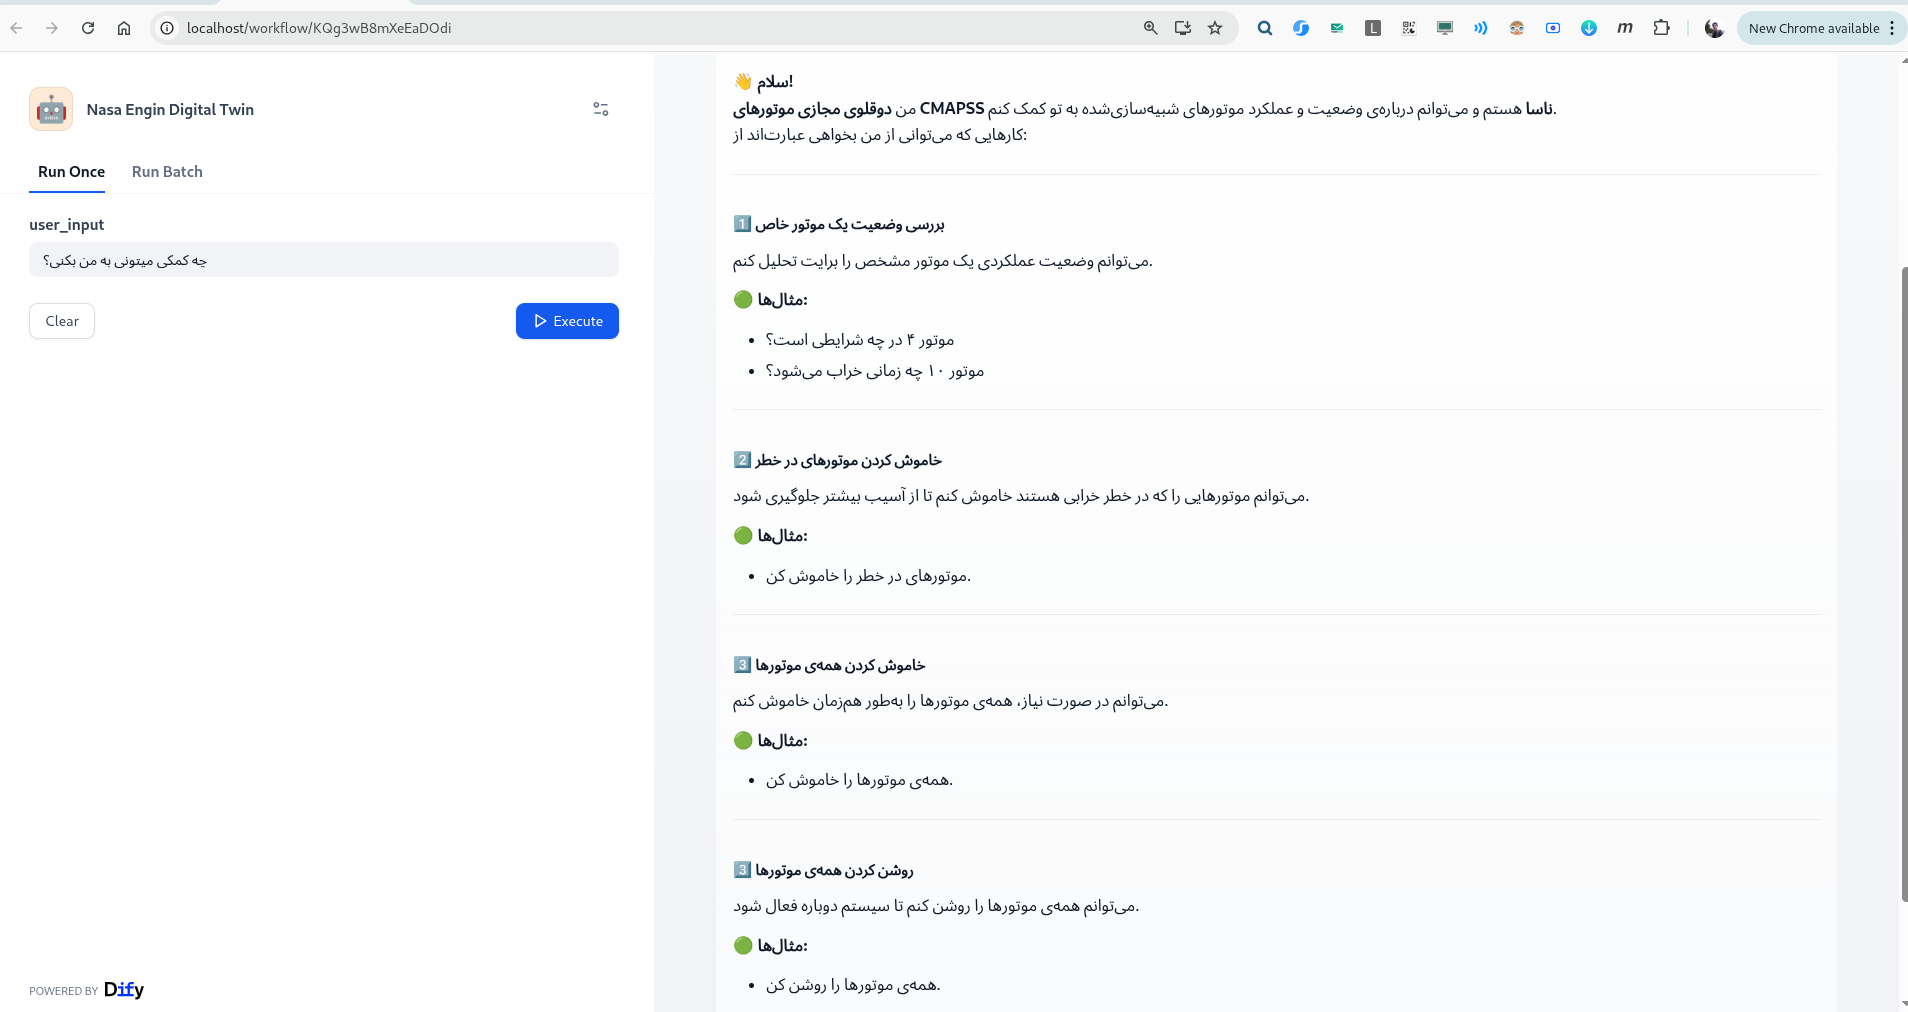
\includegraphics[width=0.85\textwidth]{images/llm_help_response.png}
	\caption{پاسخ عامل زبانی به پرسش معرفی قابلیت‌ها (شاخه راهنما): فهرست ساختاریافته چهار قابلیت اصلی با مثال‌های کاربردی نمایش داده می‌شود؛ این شاخه بدون فراخوانی \gls{LLM} اجرا می‌شود}
	\label{fig:llm-help}
\end{figure}

نمونه دوم موتور ۱ است که با \gls{RUL}=۱۶۴٫۶۷ چرخه (بسیار بیشتر از آستانه ۳۰) در وضعیت عادی قرار دارد. پاسخ عامل شامل شناسایی وضعیت عادی، معرفی حسگرهای \lr{T30}، \lr{Ps30} و \lr{NRf} به‌عنوان مؤثرترین حسگرها و توصیه «ادامه پرواز با نظارت دقیق» است.

نمونه سوم موتور ۲۴ با \gls{RUL}=۲۷٫۴۱ چرخه است که از آستانه بحران ($30$) گذشته. شکل \ref{fig:llm-engine-query} نمونه‌ای از این نوع پاسخ را نشان می‌دهد. در این حالت، عامل پنج حسگر مؤثر را با تفسیر فیزیکی توضیح می‌دهد: \lr{Ps30} با افزایش فشار استاتیک در خروجی \lr{HPC} نشانه فرسودگی را ثبت کرده، \lr{T30} دمای بالاتر از حد عادی را در خروجی \lr{HPC} نمایش می‌دهد، \lr{T24} کاهش کارایی در ورودی \lr{LPC} را نشان می‌دهد و \lr{BPR} و \lr{phi} نیز تغییرات غیرعادی در سامانه‌های کنترل و سوخت را گزارش می‌کنند. توصیه عملیاتی قاطع است: \textbf{بازرسی فوری}.

\begin{figure}[H]
	\centering
	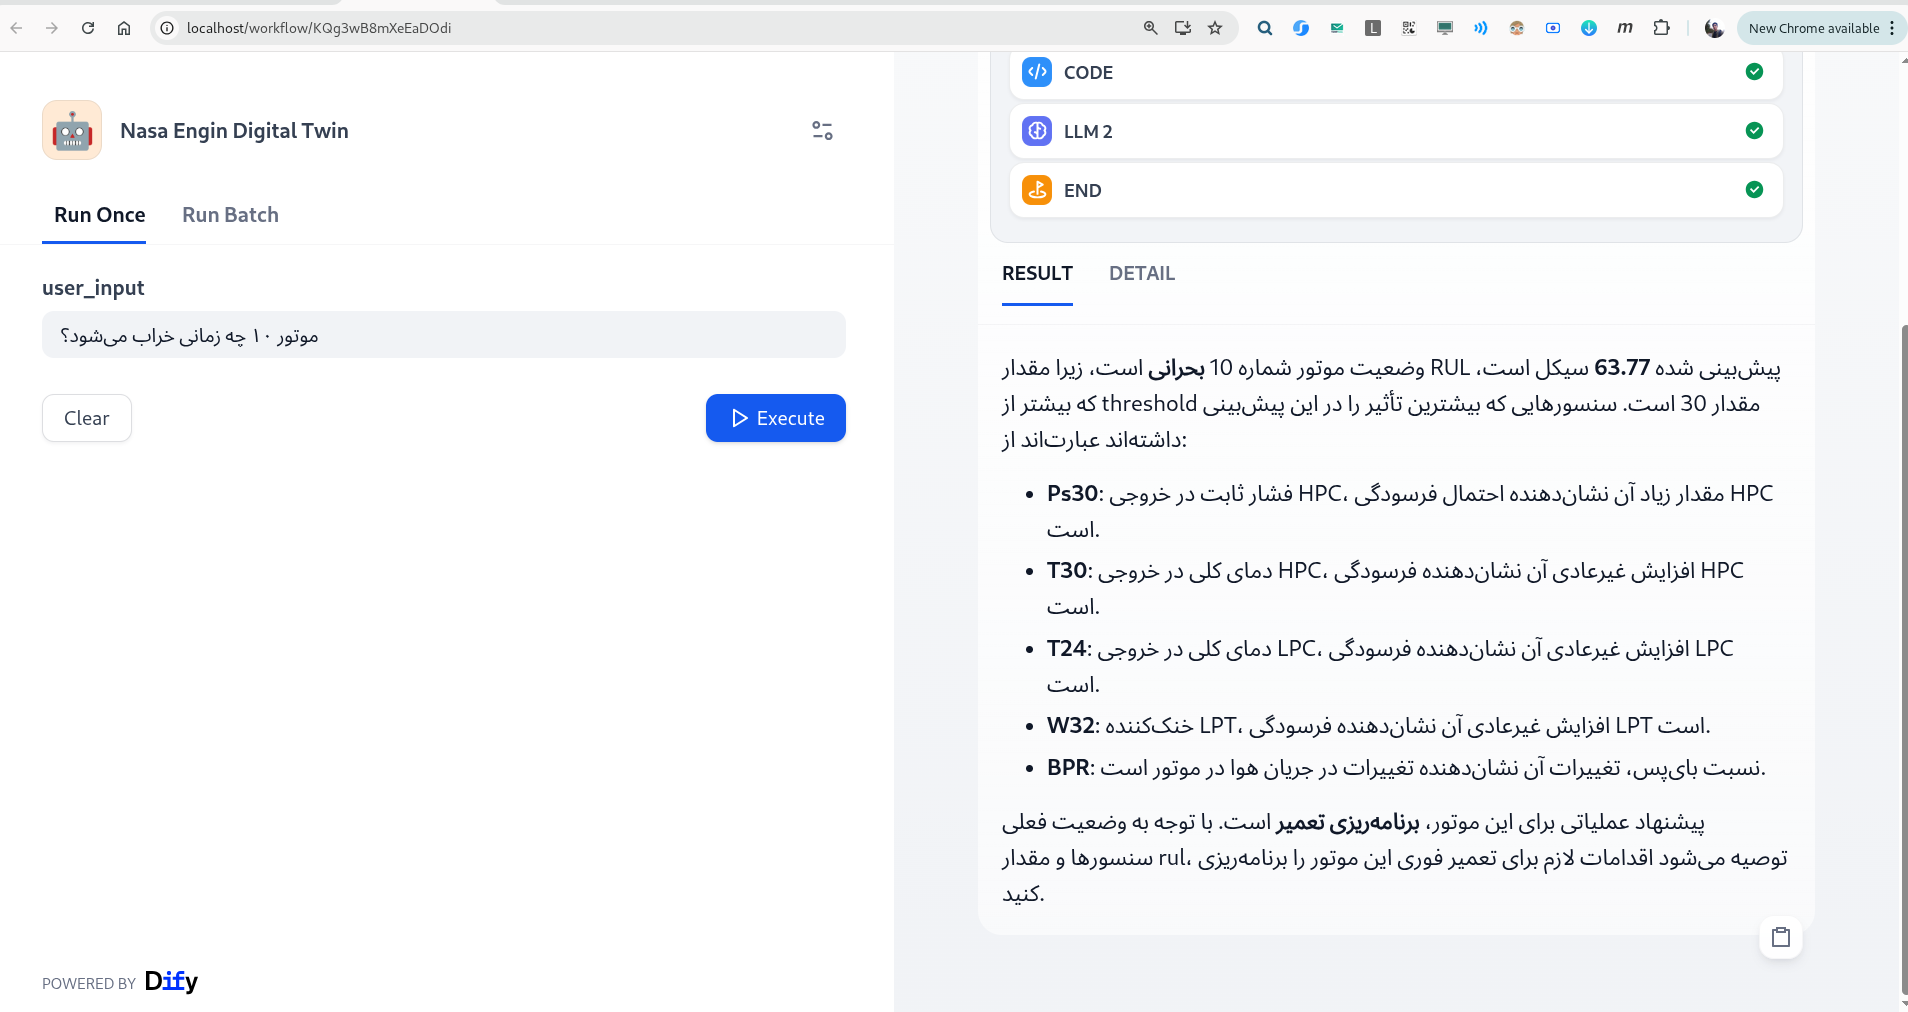
\includegraphics[width=0.85\textwidth]{images/llm_engine10_query.png}
	\caption{نمونه پاسخ عامل زبانی برای پرس‌وجوی وضعیت موتور: ساختار سه‌بخشی پاسخ (وضعیت، حسگرهای مؤثر با تفسیر فیزیکی، توصیه عملیاتی) قابل مشاهده است}
	\label{fig:llm-engine-query}
\end{figure}


% -----------------------------------------------------------------------
\section{عامل پایش بی‌درنگ}\label{sec:impl-monitor}

\subsection{سازوکار شبیه‌سازی جریان داده}

چالش اصلی در پیاده‌سازی عامل پایش این است که داده \gls{CMAPSS} یک فایل ثابت است، نه یک جریان داده زنده. راه‌حل طراحی‌شده، شبیه‌سازی پیشرفت زمان از طریق ساعت منطقی است. عامل پایش یک متغیر $t_\mathrm{clock}$ نگه‌داری می‌کند که با هر تیک حلقه به‌اندازه $\Delta t$ افزایش می‌یابد:

\begin{equation}
t_{\mathrm{clock}} \leftarrow t_{\mathrm{clock}} + \Delta t
\end{equation}

در هر تیک، این ساعت منطقی به عامل پیش‌بینی ارسال می‌شود:
\begin{latin}
\begin{verbatim}
GET /api/predict/engines_with_low_rul/?threshold=θ&until_clock=t
\end{verbatim}
\end{latin}

پارامتر \lr{until\_clock} به عامل پیش‌بینی می‌گوید که برای هر موتور تنها داده تا چرخه $t$ را در نظر بگیرد. بدین ترتیب، وقتی ساعت منطقی پیش می‌رود، موتورهایی که تعداد چرخه بیشتری داده دارند وارد پنجره پیش‌بینی می‌شوند و مقدار \gls{RUL} آن‌ها کاهش می‌یابد؛ دقیقاً همان‌طور که در یک سامانه واقعی بی‌درنگ داده می‌رسد. همان‌طور که در شکل \ref{fig:impl-monitor-arch} نشان داده شده است، این \gls{Mechanism} در یک حلقه با دو بخش اصلی پیاده‌سازی شده است: سمت چپ حلقه شبیه‌سازی زمان و اجرای درخواست \lr{API} است؛ سمت راست رابط کاربری است که موتورهای با \gls{RUL} کمتر از آستانه را در کارت‌های رنگی نمایش می‌دهد.

\begin{figure}[H]
	\centering
	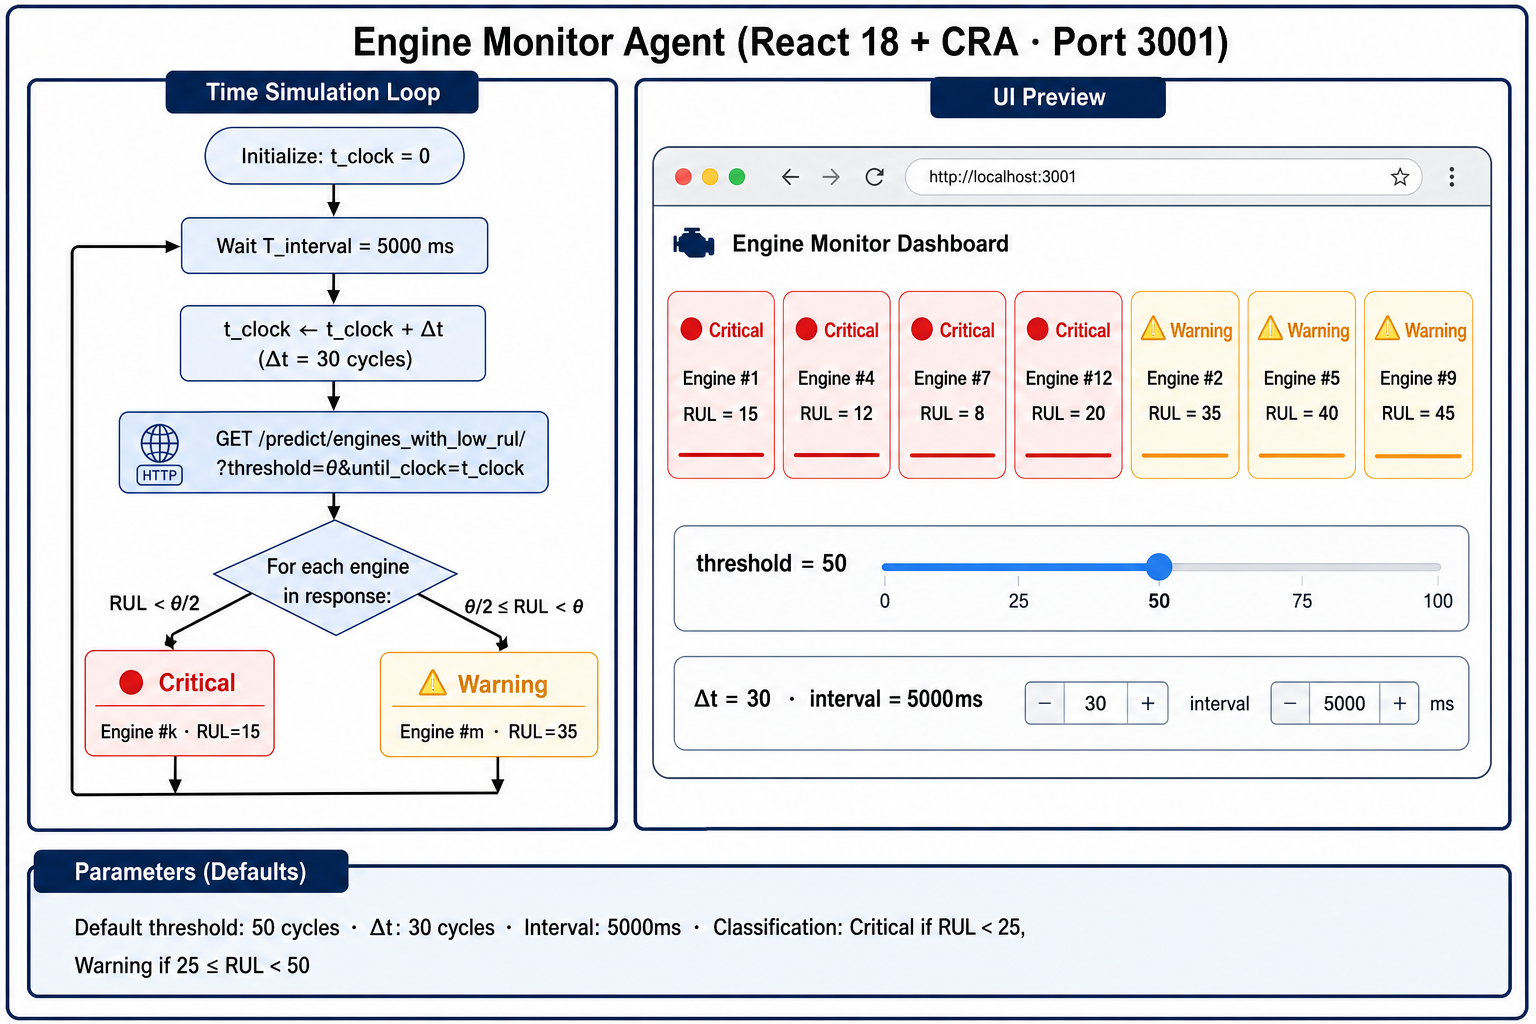
\includegraphics[width=0.95\textwidth]{images/agent_engine_monitor.png}
	\caption{معماری عامل پایش بی‌درنگ: حلقه شبیه‌سازی زمان (سمت چپ) ساعت منطقی را هر ۵ ثانیه به‌اندازه ۳۰ چرخه پیش می‌برد و نتیجه را در رابط کارت‌محور (سمت راست) به کاربر نمایش می‌دهد؛ کارت‌های نارنجی هشدار و کارت‌های قرمز وضعیت بحرانی را نشان می‌دهند}
	\label{fig:impl-monitor-arch}
\end{figure}

\subsection{پارامترها و رابط کاربری}

سه پارامتر اصلی عملکرد عامل پایش را تعیین می‌کنند. آستانه $\theta$ مرز ورود به فهرست پایش را مشخص می‌کند: موتوری که \gls{RUL} آن از $\theta$ کمتر باشد کارت دریافت می‌کند. گام $\Delta t$ سرعت پیشرفت شبیه‌سازی را کنترل می‌کند؛ مقدار پیش‌فرض ۳۰ چرخه یعنی هر ۵ ثانیه معادل ۳۰ چرخه از عمر موتور گذشته است. آستانه بحرانی $\theta/2$ مرز تفکیک کارت‌های هشدار (نارنجی) از بحرانی (قرمز) است. این سه پارامتر در جدول \ref{tab:monitor-params} با مقادیر پیش‌فرض و نقش هر کدام توضیح داده شده‌اند.

\begin{table}[ht]
	\centering
	\caption{پارامترهای پیش‌فرض عامل پایش بی‌درنگ}
	\label{tab:monitor-params}
	\begin{tabular}{p{4cm}p{3cm}p{6.5cm}}
		\toprule
		\textbf{پارامتر} & \textbf{پیش‌فرض} & \textbf{توضیح} \\
		\midrule
		\lr{threshold} ($\theta$) & ۵۰ چرخه & آستانه ورود به فهرست پایش \\
		\lr{step} ($\Delta t$) & ۳۰ چرخه & گام پیشرفت ساعت شبیه‌سازی \\
		\lr{interval} & ۵۰۰۰ میلی‌ثانیه & دوره تکرار حلقه \\
		آستانه بحرانی & $\theta / 2 = 25$ & مرز تفکیک هشدار/بحرانی \\
		\bottomrule
	\end{tabular}
\end{table}

ساختار کد سرویس از معماری مؤلفه‌محور \lr{React} پیروی می‌کند:
\begin{latin}
\begin{verbatim}
engine-monitor/
├── src/
│   ├── App.js           # simulation loop (Start/Stop/clock)
│   ├── services/api.js  # fetchEngineData, demo fallback
│   ├── utils/constants.js
│   └── components/
│       ├── Dashboard/   # EngineCard, StatsPanel
│       └── Config/ConfigModal.js
└── docker-compose.yaml  # port 3001
\end{verbatim}
\end{latin}

شکل \ref{fig:monitor-ui-on} رابط کاربری عامل پایش را در حالت فعال نشان می‌دهد. در این تصویر، پس از روشن شدن همه موتورها و پیشرفت ساعت شبیه‌سازی، موتورهایی که \gls{RUL} آن‌ها از آستانه گذشته با رنگ‌های متفاوت نمایش داده می‌شوند؛ بنابراین \gls{Operator} در یک نگاه وضعیت سلامت کل ناوگان را درک می‌کند.

\begin{figure}[H]
	\centering
	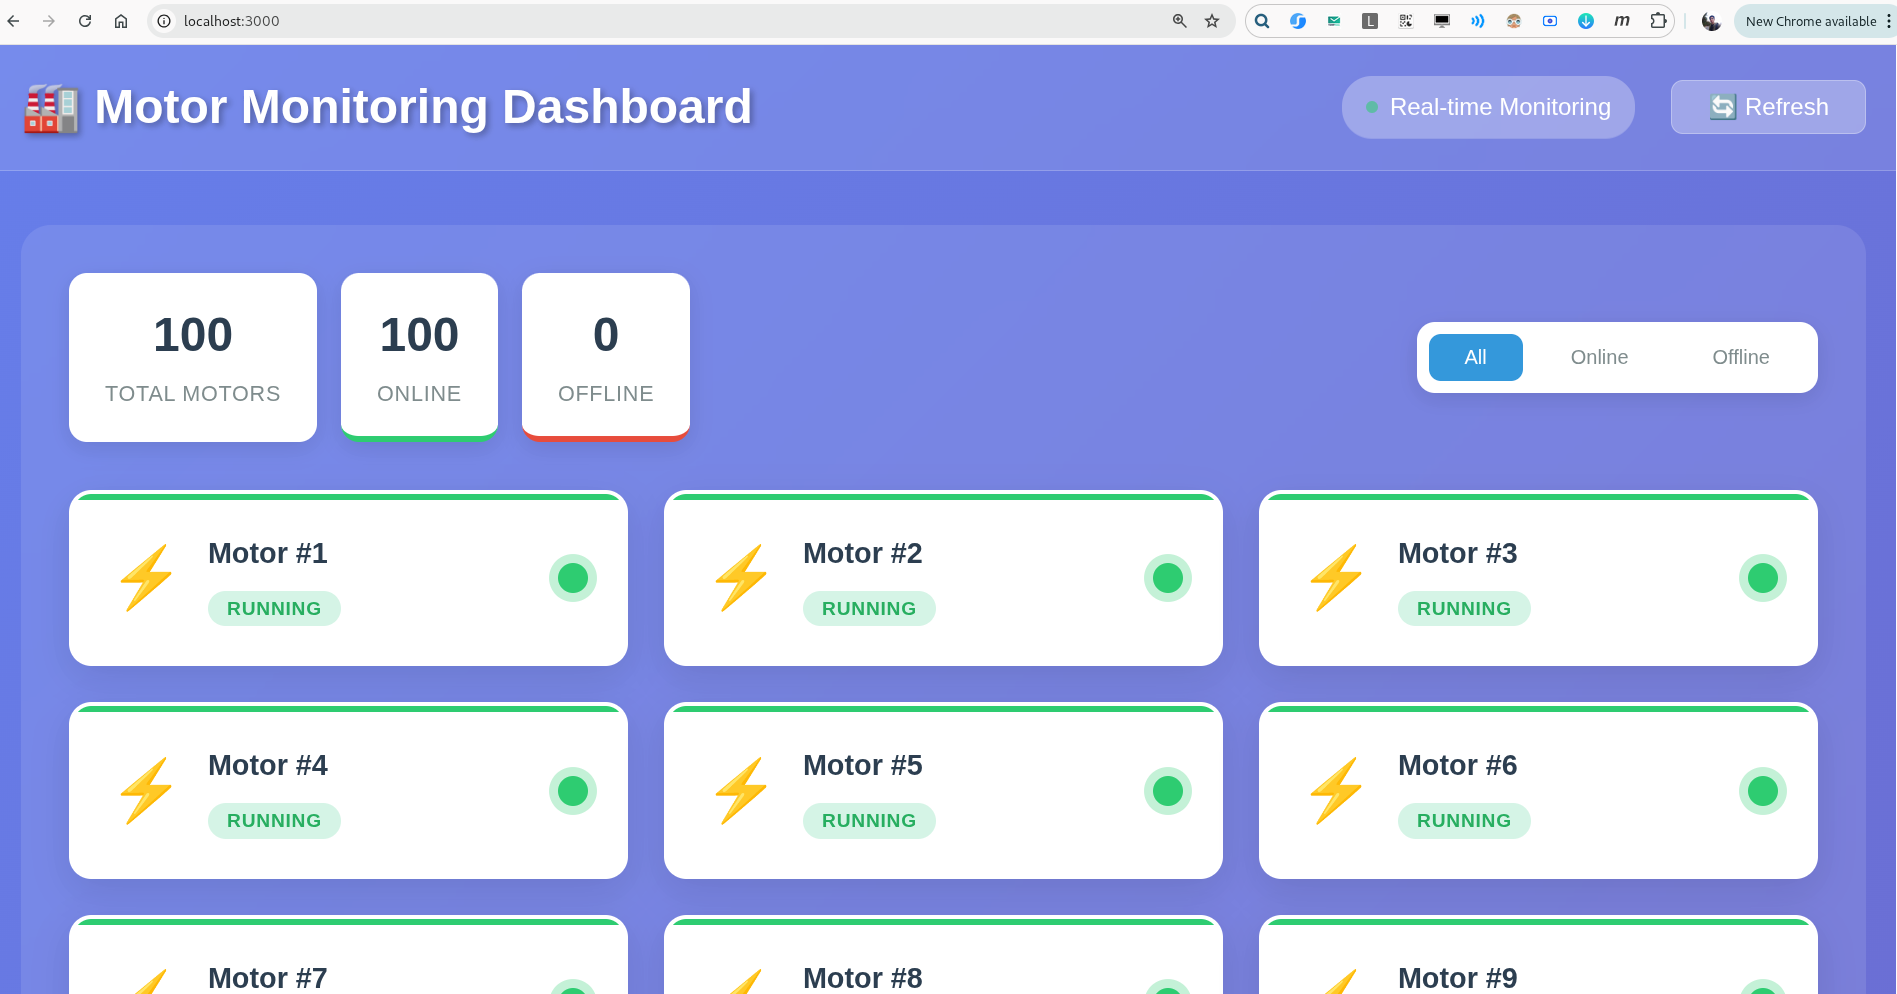
\includegraphics[width=0.92\textwidth]{images/monitor_after_on.png}
	\caption{رابط کاربری عامل پایش در حالت فعال پس از روشن شدن همه موتورها: کارت‌های نارنجی موتورهای در مرحله هشدار ($25 \le \mathrm{RUL} < 50$) و کارت‌های قرمز موتورهای در وضعیت بحرانی ($\mathrm{RUL} < 25$) را نشان می‌دهند}
	\label{fig:monitor-ui-on}
\end{figure}

شکل \ref{fig:dashboard-sim-input} تنظیمات شبیه‌سازی را نشان می‌دهد. \gls{Operator} می‌تواند گام زمانی $\Delta t$ و دوره تکرار حلقه را تنظیم کند تا سرعت شبیه‌سازی را با نیاز \gls{Demo} یا آزمایش تطبیق دهد. این قابلیت پیکربندی زنده یکی از نکات ارزشمند در طراحی رابط کاربری است.

\begin{figure}[H]
	\centering
	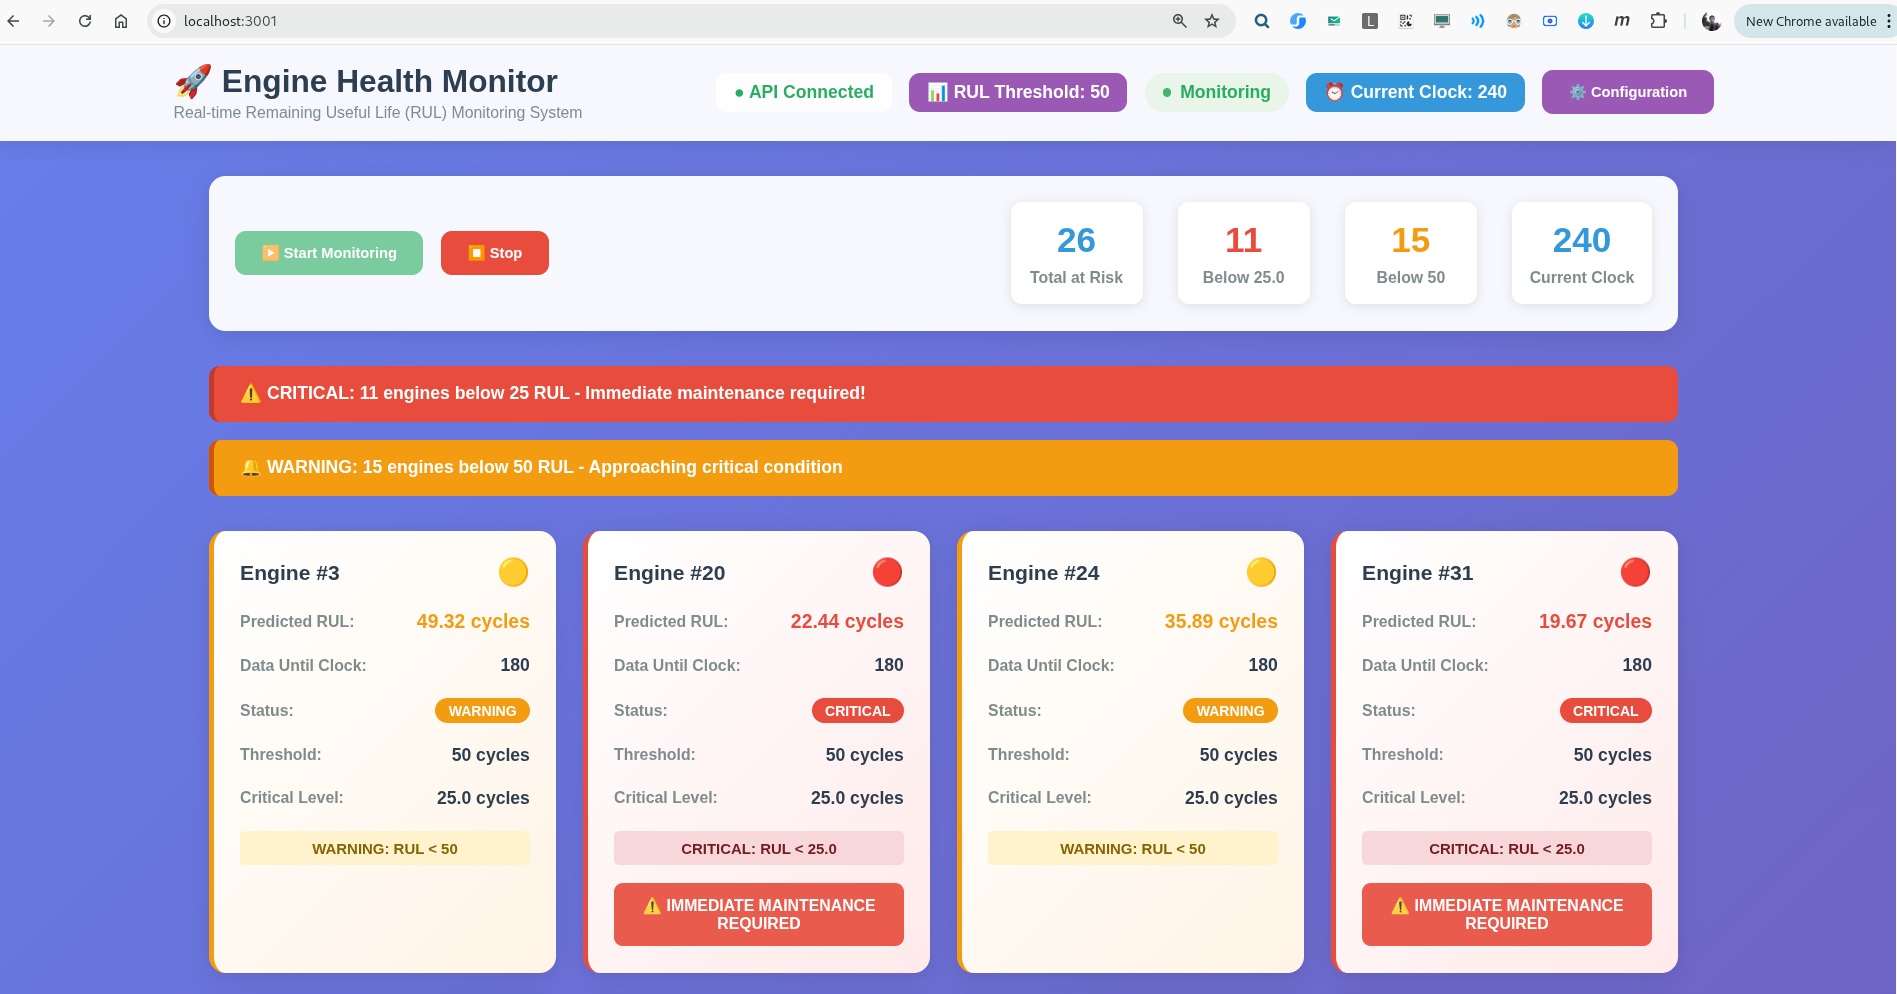
\includegraphics[width=0.85\textwidth]{images/dashboard_sim_input.png}
	\caption{رابط تنظیمات شبیه‌سازی ورودی داده: \gls{Operator} می‌تواند گام زمانی ($\Delta t$) و دوره تکرار حلقه را در حین اجرا تنظیم کند تا سرعت شبیه‌سازی با سناریوی مورد نظر تطبیق یابد}
	\label{fig:dashboard-sim-input}
\end{figure}

یک ویژگی مقاومتی در طراحی این سرویس وجود دارد: در صورت قطع ارتباط با عامل پیش‌بینی، یک \gls{Mechanism} \lr{fallback} داده \gls{Demo} تولید می‌کند تا رابط کاربری خالی نماند. این رفتار برای \glspl{Demo} و محیط‌های توسعه مناسب است و باید در استقرار تولیدی غیرفعال شود.


% -----------------------------------------------------------------------
\section{عامل تابلو وضعیت}\label{sec:impl-dashboard}

عامل \gls{Dashboard} نقش «آینه شفاف» ناوگان را ایفا می‌کند. برخلاف عامل پایش که خود داده پیش‌بینی را درخواست می‌کند، این عامل کاملاً فقط‌خواندنی است و هیچ استنتاج یا فرمانی صادر نمی‌کند. وظیفه اصلی آن نمایش بصری اثر فرمان‌های عامل زبانی روی وضعیت ناوگان است؛ بدین ترتیب \gls{Operator} می‌تواند بلافاصله تأثیر دستوری که داده را با چشمان خود ببیند.

\begin{figure}[H]
	\centering
	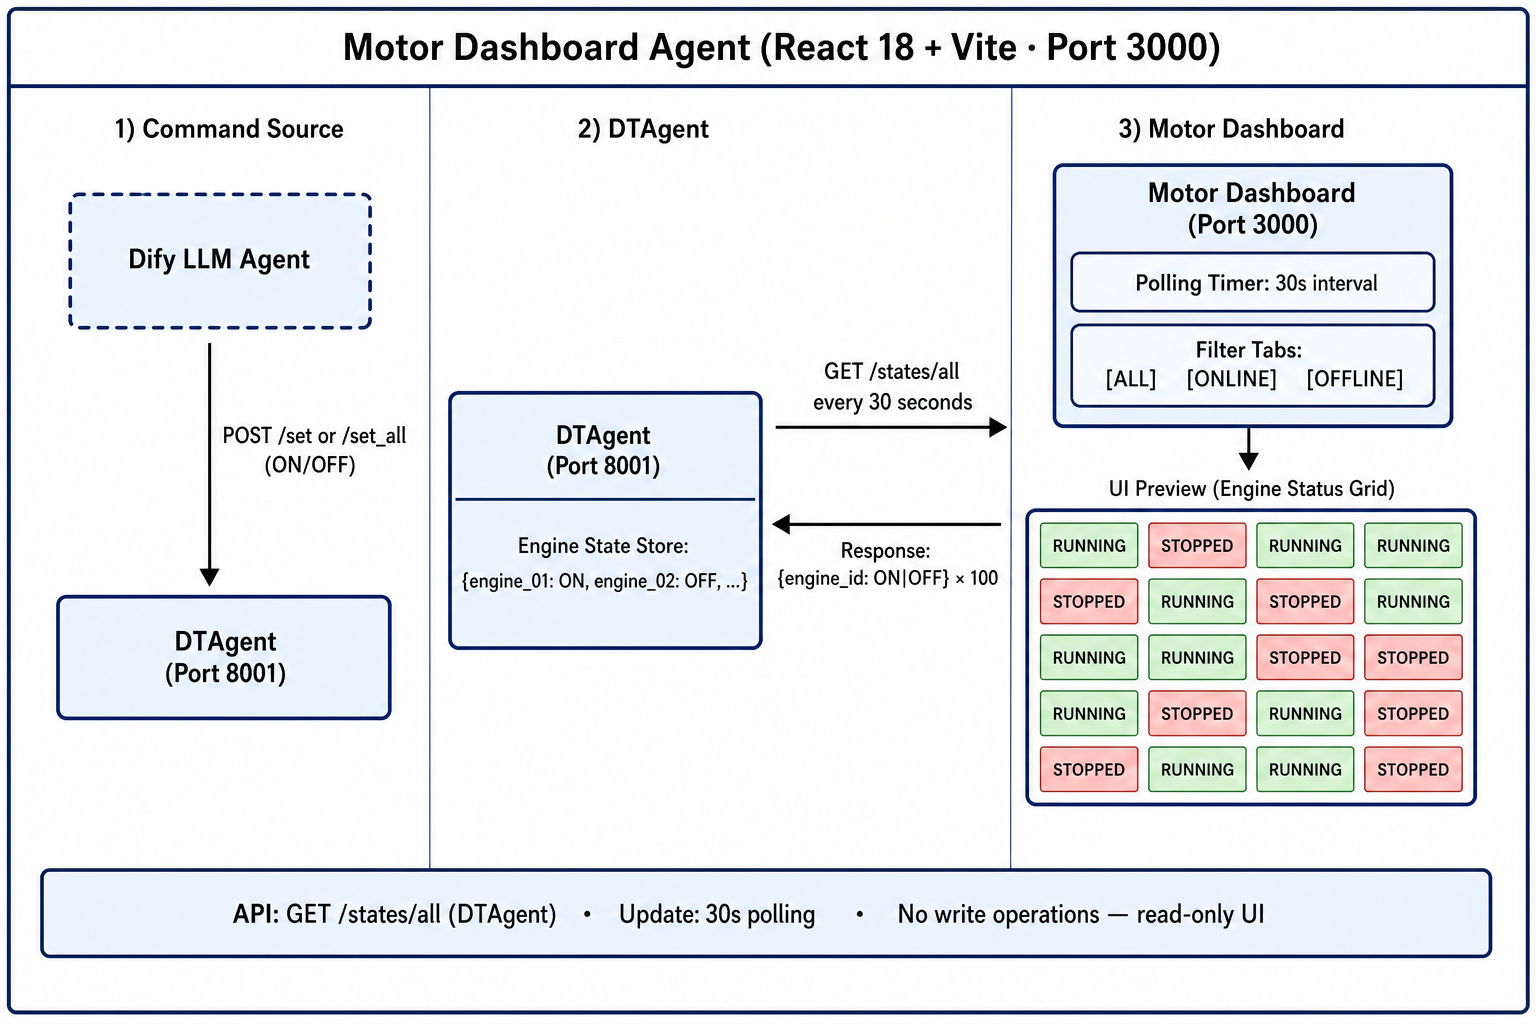
\includegraphics[width=0.90\textwidth]{images/agent_motor_dashboard.png}
	\caption{معماری عامل \gls{Dashboard}: جریان اطلاعات تنها از عامل دوقلو به \gls{Dashboard} است (فلش تک‌جهته)؛ جریان فرمان از عامل زبانی به عامل دوقلو ارسال می‌شود و \gls{Dashboard} این تغییر را در نظرسنجی بعدی دریافت می‌کند}
	\label{fig:impl-dashboard-arch}
\end{figure}

الگوی نظرسنجی دوره‌ای ۳۰ ثانیه‌ای انتخاب‌شده تعادلی بین تازگی اطلاعات و بار شبکه است. در یک سامانه پیام‌رسان واقعی، می‌توان از \lr{WebSocket} یا \lr{Server-Sent Events} برای اعلان‌های آنی استفاده کرد، اما در بستر آزمایشگاهی، نظرسنجی دوره‌ای کافی و پیاده‌سازی ساده‌تری است. سه فیلتر \lr{ALL}، \lr{ONLINE} و \lr{OFFLINE} به \gls{Operator} امکان می‌دهند روی زیرمجموعه خاصی از ناوگان تمرکز کند؛ این ویژگی در ناوگان‌های بزرگ‌تر بسیار مفیدتر می‌شود.

ساختار کد از معماری مؤلفه‌ای \lr{React} با جداسازی منطق دریافت داده از نمایش پیروی می‌کند:
\begin{latin}
\begin{verbatim}
motor-dashboard/
├── src/
│   ├── App.jsx              # polling loop + Retry
│   ├── services/api.js      # getMotorStates → /states/all
│   └── components/
│       ├── MotorGrid/       # filter + stats
│       └── MotorCard/       # RUNNING/STOPPED card
└── docker-compose.yaml      # port 3000
\end{verbatim}
\end{latin}

تأخیر بازخورد این سرویس تا ۳۰ ثانیه (دوره نظرسنجی) است. در \glspl{Demo} که تغییر وضعیت ناوگان باید بلافاصله دیده شود، ممکن است \lr{Refresh} دستی لازم باشد؛ این رفتار نه یک اشکال، بلکه پیامد عمداً انتخاب‌شده الگوی نظرسنجی است.


% -----------------------------------------------------------------------
\section{سناریوی سرتاسری یکپارچه}\label{sec:impl-e2e}

برای نشان دادن انسجام کل سامانه، دو سناریوی مکمل ارائه می‌شود که روی هم کل قابلیت‌های سامانه را پوشش می‌دهند.

\subsection{سناریو الف --- پرس‌وجوی وضعیت موتور}

در این سناریو، \gls{Operator} می‌خواهد وضعیت سلامت یک موتور مشخص را با زبان طبیعی بپرسد. کاربر جمله‌ای فارسی را در رابط \lr{Dify} وارد می‌کند. طبقه‌بند نیت \lr{gpt-4o-mini} آن را به کلاس ۱ (وضعیت یک موتور) تعیین می‌کند. یک \gls{LLM} سبک شناسه موتور را از جمله کاربر استخراج می‌کند و گره \lr{HTTP} از عامل پیش‌بینی درخواست پیش‌بینی می‌کند. پاسخ \lr{JSON} شامل \gls{RUL} و بردار اهمیت حسگرها به \gls{LLM} روایت‌گر ارسال می‌شود که پاسخ توضیح‌پذیر فارسی را می‌سازد. همان‌طور که در شکل \ref{fig:seq-rul-query} مشاهده می‌شود، جریان اطلاعاتی از کاربر به عامل پیش‌بینی و بازگشت آن در قالب روایت فارسی در یک چرخه کامل انجام می‌شود.

\begin{figure}[H]
	\centering
	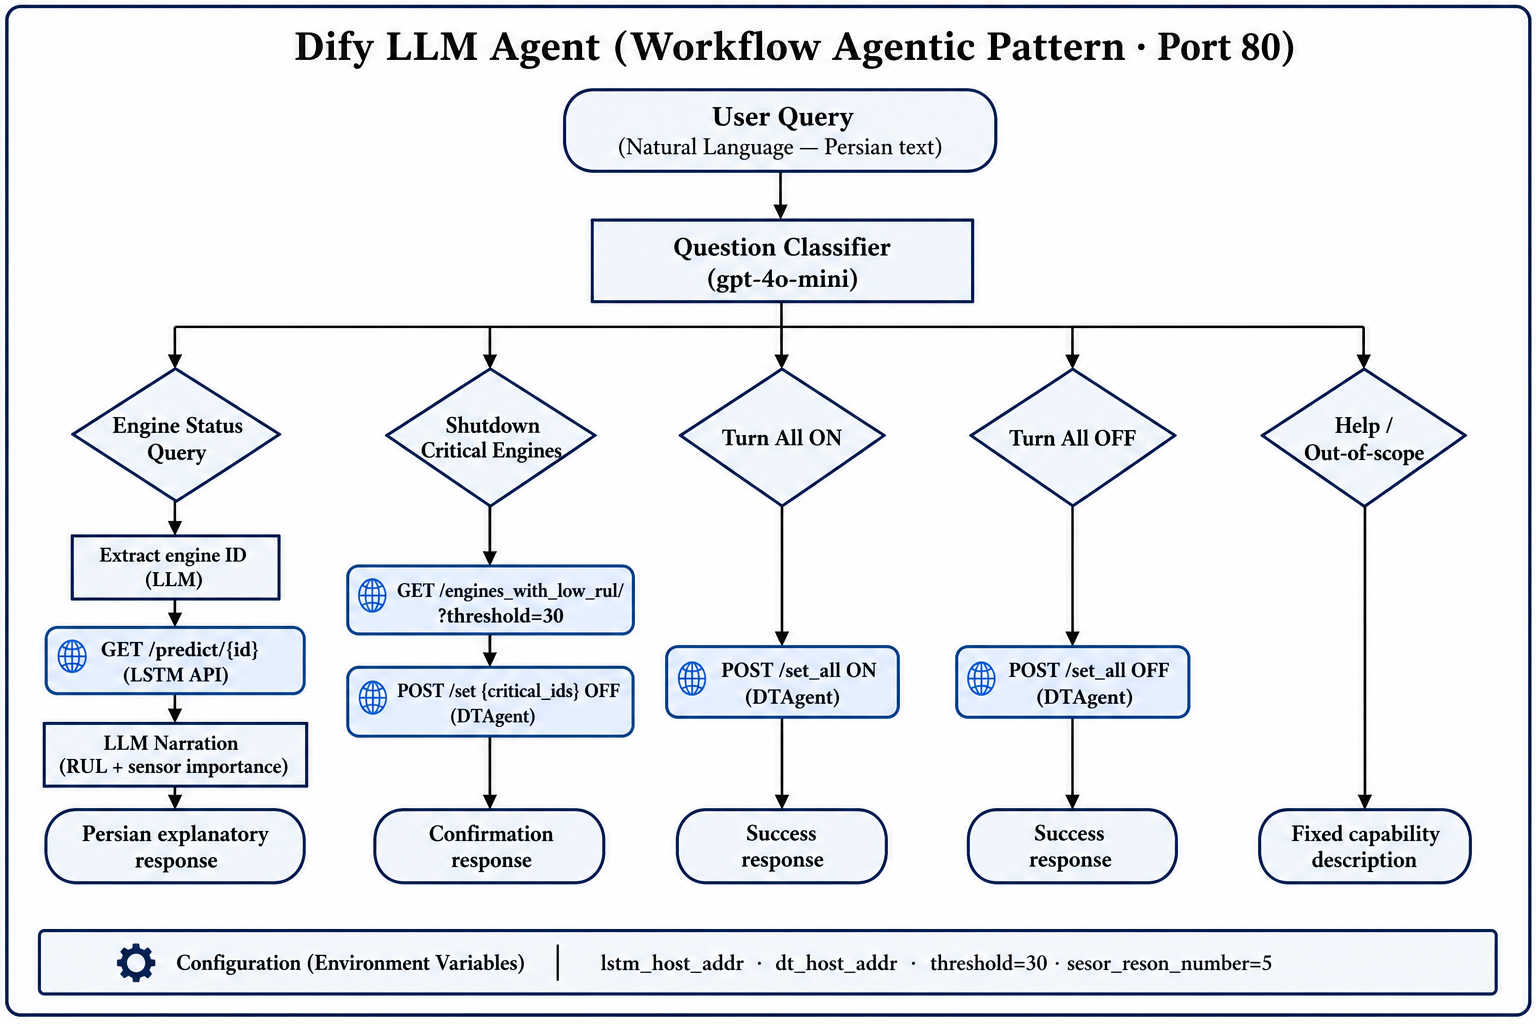
\includegraphics[width=0.90\textwidth]{images/agent_dify_llm.png}
	\caption{\gls{Workflow} عامل زبانی در سناریوی پرس‌وجوی وضعیت موتور: از طبقه‌بندی نیت تا روایت فارسی، هر گره وظیفه مشخصی دارد؛ \gls{LLM} تنها در دو گره استفاده می‌شود \cite{CHEN2025102982LLMDT}}
	\label{fig:seq-rul-query}
\end{figure}

\subsection{سناریو ب --- خاموش‌سازی موتورهای در خطر}

این سناریو حلقه کنترل بسته را به نمایش می‌گذارد. کاربر با یک دستور فارسی فرمان می‌دهد که موتورهای در خطر خاموش شوند. عامل زبانی بدون هیچ مکالمه اضافی، ابتدا از عامل پیش‌بینی فهرست موتورهای با \gls{RUL} پایین را دریافت می‌کند، سپس شناسه این موتورها را به عامل دوقلو ارسال و فرمان \lr{OFF} صادر می‌کند. شکل \ref{fig:seq-shutdown} پاسخ موفقیت این عملیات را نشان می‌دهد. مهم‌تر از پاسخ متنی، تأثیر واقعی این فرمان است: در نظرسنجی بعدی عامل \gls{Dashboard}، موتورهای خاموش‌شده با رنگ قرمز «STOPPED» دیده می‌شوند و در تیک بعدی عامل پایش، کارت‌های آن موتورها از صفحه ناپدید می‌شوند --- زیرا موتوری که خاموش شده دیگر در فهرست «موتورهای فعال با \gls{RUL} پایین» قرار نمی‌گیرد.

\begin{figure}[H]
	\centering
	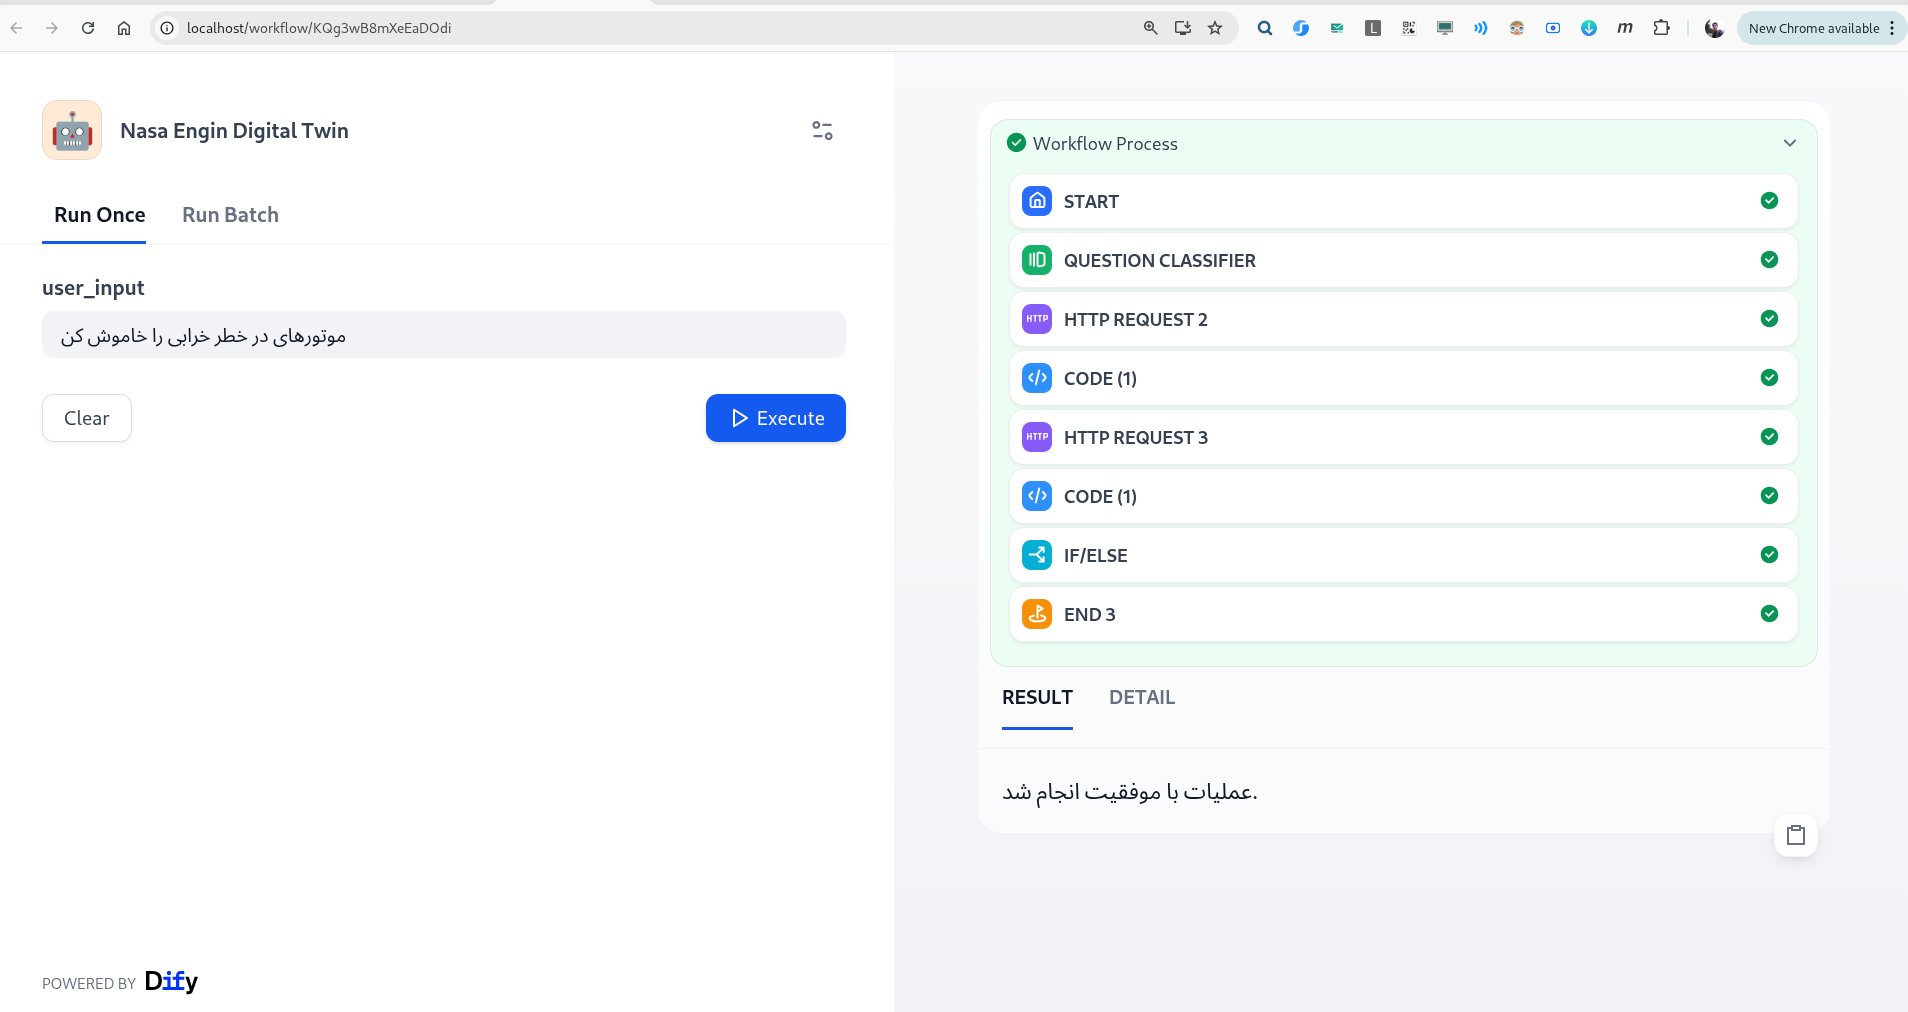
\includegraphics[width=0.85\textwidth]{images/llm_cmd_critical_off.png}
	\caption{سناریو خاموش‌سازی موتورهای در خطر: عامل زبانی پس از دریافت فهرست از عامل پیش‌بینی، فرمان \lr{OFF} را به عامل دوقلو ارسال می‌کند و تأثیر آن بلافاصله در \gls{Dashboard} و عامل پایش قابل مشاهده است}
	\label{fig:seq-shutdown}
\end{figure}


% -----------------------------------------------------------------------
\section{جمع‌بندی}\label{sec:impl-summary}

در این فصل، پیاده‌سازی کامل پنج عامل سامانه دوقلوی دیجیتال چندعاملی با تمام جزئیات فنی ارائه شد. تجربه پیاده‌سازی سه درس کلیدی به همراه داشت که به سایر پژوهشگران در پیاده‌سازی معماری‌های مشابه کمک می‌کند.

نخستین درس مربوط به الگوی خطا است. برخی نقاط پایانی کد \lr{HTTP 200} با بدنه \lr{JSON} حاوی کلید \lr{error} برمی‌گردانند. این الگوی «خطای نرم» در \glspl{Demo} راحت است چون فرآیند \lr{crash} نمی‌کند، اما ردیابی مشکلات را دشوار می‌کند. راه‌حل اتخاذشده این بود که عامل زبانی علاوه بر کد وضعیت، بدنه پاسخ را نیز با یک گره \lr{Code} بررسی کند.

درس دوم به وضعیت \lr{in-memory} مربوط است. نگه‌داری وضعیت \lr{ON/OFF} موتورها در حافظه فرآیند به ظاهر ساده است، اما یک پیامد مهم دارد: راه‌اندازی مجدد هر \gls{Container} وضعیت را بازنشانی می‌کند. در محیط آزمایشگاهی این رفتار مطلوب است چون هر اجرای \gls{Demo} از حالت شناخته‌شده آغاز می‌شود؛ اما در استقرار صنعتی، پایداری با \lr{Redis} یا یک پایگاه داده مستمر ضروری است.

سومین درس به ناهماهنگی پیکربندی مربوط می‌شود. آستانه پیش‌فرض عامل پایش ($\theta=50$) با آستانه عامل زبانی ($\theta=30$) متفاوت است؛ این به معنای آن است که دو واسط ممکن است فهرست‌های متفاوتی از «موتورهای در خطر» نشان دهند. برای آزمایش‌های قابل‌تکرار و سازگار، باید آستانه‌ها پیش از آزمایش یکسان‌سازی شوند یا از یک پیکربندی مشترک خوانده شوند.
